% Seminar 5: Selecția Modelului și Backtesting

\documentclass[9pt, aspectratio=169, t]{beamer}
%=============================================================================
% PREAMBUL COMUN - Statistica Piețelor Financiare
% Prezentări academice de calitate Harvard
% Program de licență, Academia de Studii Economice din București
%
% Utilizare: \documentclass[9pt, aspectratio=169, t]{beamer}
%            %=============================================================================
% PREAMBUL COMUN - Statistica Piețelor Financiare
% Prezentări academice de calitate Harvard
% Program de licență, Academia de Studii Economice din București
%
% Utilizare: \documentclass[9pt, aspectratio=169, t]{beamer}
%            %=============================================================================
% PREAMBUL COMUN - Statistica Piețelor Financiare
% Prezentări academice de calitate Harvard
% Program de licență, Academia de Studii Economice din București
%
% Utilizare: \documentclass[9pt, aspectratio=169, t]{beamer}
%            \input{preamble}
%            \subtitle{Seminar X: Titlul Seminarului}
%            \begin{document} ...
%=============================================================================

% Asigură încadrarea conținutului pe diapozitive
\setbeamersize{text margin left=8mm, text margin right=8mm}

%=============================================================================
% CONFIGURARE TEMĂ ȘI STIL
%=============================================================================
\usetheme{default}

% Paletă de Culori
\definecolor{MainBlue}{RGB}{26, 58, 110}
\definecolor{AccentBlue}{RGB}{26, 58, 110}
\definecolor{IDAred}{RGB}{205, 0, 0}
\definecolor{DarkGray}{RGB}{51, 51, 51}
\definecolor{MediumGray}{RGB}{128, 128, 128}
\definecolor{LightGray}{RGB}{248, 248, 248}
\definecolor{VeryLightGray}{RGB}{235, 235, 235}
\definecolor{KeynoteGray}{RGB}{218, 218, 218}
\definecolor{SectionGray}{RGB}{120, 120, 120}
\definecolor{FooterGray}{RGB}{100, 100, 100}
\definecolor{Crimson}{RGB}{220, 53, 69}
\definecolor{Forest}{RGB}{46, 125, 50}
\definecolor{Amber}{RGB}{181, 133, 63}
\definecolor{Orange}{RGB}{230, 126, 34}
\definecolor{Purple}{RGB}{142, 68, 173}

% Fundal gradient (gradient Keynote exact 315°: alb la RGB 218,218,218)
\setbeamertemplate{background}{%
    \begin{tikzpicture}[remember picture, overlay]
        \shade[shading=axis, shading angle=315,
        top color=white, bottom color=KeynoteGray]
        (current page.south west) rectangle (current page.north east);
    \end{tikzpicture}%
}
% Culoare solidă de rezervă pentru compatibilitate
\setbeamercolor{background canvas}{bg=}

\setbeamercolor{palette primary}{bg=MainBlue, fg=white}
\setbeamercolor{palette secondary}{bg=MainBlue!85, fg=white}
\setbeamercolor{palette tertiary}{bg=MainBlue!70, fg=white}
\setbeamercolor{structure}{fg=MainBlue}
\setbeamercolor{title}{fg=IDAred}
\setbeamercolor{frametitle}{fg=IDAred, bg=}
\setbeamercolor{block title}{bg=MainBlue, fg=white}
\setbeamercolor{block body}{bg=VeryLightGray, fg=DarkGray}
\setbeamercolor{block title alerted}{bg=Crimson, fg=white}
\setbeamercolor{block body alerted}{bg=Crimson!8, fg=DarkGray}
\setbeamercolor{block title example}{bg=Forest, fg=white}
\setbeamercolor{block body example}{bg=Forest!8, fg=DarkGray}
\setbeamercolor{item}{fg=MainBlue}

% Font institute mai mic pentru a evita overfull hbox pe pagina de titlu
\setbeamerfont{institute}{size=\footnotesize}

% Culori subsol
\setbeamercolor{author in head/foot}{fg=FooterGray, bg=}
\setbeamercolor{title in head/foot}{fg=FooterGray, bg=}
\setbeamercolor{date in head/foot}{fg=FooterGray, bg=}
\setbeamercolor{section in head/foot}{fg=FooterGray, bg=}
\setbeamercolor{subsection in head/foot}{fg=FooterGray, bg=}

% Stiluri marcatori
\setbeamertemplate{itemize item}{\color{MainBlue}$\boxdot$}
\setbeamertemplate{itemize subitem}{\color{MainBlue}$\blacktriangleright$}
\setbeamertemplate{itemize subsubitem}{\color{MainBlue}\tiny$\bullet$}
\setbeamertemplate{itemize/enumerate body begin}{\normalsize}
\setbeamertemplate{itemize/enumerate subbody begin}{\normalsize}

% Stiluri cuprins (bullets în loc de numere)
\setbeamertemplate{section in toc}{%
    \leavevmode\leftskip=1.5em%
    \llap{\color{MainBlue}$\boxdot$\kern0.5em}%
    \inserttocsection\par%
}

% Spațiere compactă
\setlength{\leftmargini}{10pt}
\setlength{\leftmarginii}{10pt}
\makeatletter
\def\@listi{\leftmargin\leftmargini \topsep 0pt \parsep 0pt \itemsep 0pt}
\def\@listii{\leftmargin\leftmarginii \topsep 0pt \parsep 0pt \itemsep 0pt}
\makeatother

\setbeamertemplate{navigation symbols}{}

%=============================================================================
% ANTET PERSONALIZAT
%=============================================================================
\setbeamertemplate{headline}{%
    \vskip10pt%
    \hbox to \paperwidth{%
        \hskip0.5cm%
        {\small\color{FooterGray}\renewcommand{\hyperlink}[2]{##2}\insertsectionhead}%
        \hfill%
        \textcolor{FooterGray}{\small\insertframenumber}%
        \hskip0.5cm%
    }%
    \vskip4pt%
    {\color{FooterGray}\hrule height 0.4pt}%
}

%=============================================================================
% SUBSOL PERSONALIZAT
%=============================================================================
\usepackage{fontawesome5}

\setbeamertemplate{footline}{%
    {\color{FooterGray}\hrule height 0.4pt}%
    \vskip4pt%
    \hbox to \paperwidth{%
        \hskip0.5cm%
        \textcolor{FooterGray}{\small Statistica Piețelor Financiare}%
        \hfill%
        \raisebox{-0.1em}{%
            \begin{tikzpicture}[x=0.08em, y=0.08em, line width=0.4pt]
                \draw[FooterGray] (0,3) -- (1,4) -- (2,3.5) -- (3,5) -- (4,4) -- (5,6) -- (6,5.5) -- (7,4) -- (8,5) -- (9,7) -- (10,6) -- (11,5) -- (12,6.5) -- (13,8) -- (14,7) -- (15,6) -- (16,7.5) -- (17,9) -- (18,8) -- (19,7) -- (20,8.5) -- (21,10) -- (22,9) -- (23,8) -- (24,9.5);
            \end{tikzpicture}%
        }%
        \hskip0.5cm%
    }%
    \vskip6pt%
}

%=============================================================================
% PACHETE
%=============================================================================
\usepackage[utf8]{inputenc}
\usepackage[T1]{fontenc}
\usepackage{amsmath, amssymb, amsthm}
\usepackage{mathtools}
\usepackage{bm}
\usepackage{tikz}
\usetikzlibrary{arrows.meta, positioning, shapes, calc, decorations.pathreplacing, shadings}
\usepackage{booktabs}
\usepackage{multirow}
\usepackage{array}
\usepackage{graphicx}
\usepackage{hyperref}
\usepackage{colortbl}
\usepackage{listings}
\lstset{basicstyle=\ttfamily\small, breaklines=true, frame=single, backgroundcolor=\color{VeryLightGray}}
\hypersetup{colorlinks=true, linkcolor=MainBlue, urlcolor=MainBlue}
\graphicspath{{../../logos/}{../../charts/}{../../photos/}}
\hfuzz=2pt
\vfuzz=2pt

%=============================================================================
% COMANDA QUANTLET
%=============================================================================
\newcommand{\quantlet}[2]{%
    \hfill\href{#2}{%
        \raisebox{-0.15em}{
\includegraphics[height=0.7em]{ql_logo.png}}%
        \textcolor{MainBlue}{\tiny\ #1}%
    }%
}

%=============================================================================
% PAGINĂ TITLU PERSONALIZATĂ
%=============================================================================
\defbeamertemplate*{title page}{hybrid}[1][]
{
    \vspace{0.2cm}
    \begin{center}
        \href{https://www.ase.ro}{
\includegraphics[height=1.0cm]{ase_logo.png}}\hspace{0.25cm}%
        \href{https://theida.net}{
\includegraphics[height=1.0cm]{ida_logo.png}}\hspace{0.25cm}%
        \href{https://blockchain-research-center.com}{
\includegraphics[height=1.0cm]{brc_logo.png}}\hspace{0.25cm}%
        \href{https://www.ai4efin.ase.ro}{
\includegraphics[height=1.0cm]{ai4efin_logo.png}}\hspace{0.25cm}%
        \href{https://ipe.ro/new}{
\includegraphics[height=1.0cm]{acad_logo.png}}\hspace{0.25cm}%
        \href{https://www.digital-finance-msca.com}{
\includegraphics[height=1.0cm]{msca_logo.png}}%
    \end{center}

    \vspace{0.6cm}

    \begin{center}
        \begin{minipage}{0.1\textwidth}
            \centering
            \href{https://quantlet.com}{
\includegraphics[height=1.1cm]{ql_logo.png}}
        \end{minipage}%
        \begin{minipage}{0.78\textwidth}
            \centering
            {\LARGE\bfseries\usebeamercolor[fg]{title}\inserttitle}

            \vspace{0.3cm}

            {\usebeamerfont{subtitle}\usebeamercolor[fg]{title}\insertsubtitle}
        \end{minipage}%
        \begin{minipage}{0.1\textwidth}
            \centering
            \href{https://quantinar.com}{
\includegraphics[height=1.1cm]{qr_logo.png}}
        \end{minipage}
    \end{center}

    \vspace{0.6cm}

    \hspace{0.5cm}{\usebeamerfont{author}\insertauthor}

    \vspace{0.3cm}

    \hspace{0.5cm}\begin{minipage}[t]{0.9\textwidth}
        \raggedright\small\insertinstitute
    \end{minipage}
}

%=============================================================================
% MEDII PENTRU TEOREME
%=============================================================================
\theoremstyle{definition}
\setbeamertemplate{theorems}[numbered]
\newtheorem{defn}{Definiție}
\newtheorem{thm}{Teoremă}
\newtheorem{prop}{Propoziție}
\newtheorem{rmk}{Observație}

%=============================================================================
% CENTRED MINIPAGE
%=============================================================================
\newenvironment{cminipage}[1]{%
    \par\noindent\hfill\begin{minipage}{#1}\ignorespaces
}{%
    \end{minipage}\hfill\null\par
}

%=============================================================================
% COMENZI PERSONALIZATE
%=============================================================================
\newcommand{\E}{\mathbb{E}}
\newcommand{\Var}{\text{Var}}
\newcommand{\Cov}{\text{Cov}}
\newcommand{\Corr}{\text{Corr}}
\newcommand{\R}{\mathbb{R}}
\newcommand{\N}{\mathbb{N}}
\newcommand{\Z}{\mathbb{Z}}
\newcommand{\B}{\mathbf{B}}
\newcommand{\imark}{\textcolor{MainBlue}{\textbullet}}
\newcommand{\RMSE}{\text{RMSE}}
\newcommand{\MAE}{\text{MAE}}
\newcommand{\MAPE}{\text{MAPE}}
\newcommand{\correct}{\textcolor{Forest}{\checkmark}}
\newcommand{\incorrect}{\textcolor{Crimson}{\texttimes}}

%=============================================================================
% INFORMAȚII TITLU
%=============================================================================
\title[Statistica Piețelor Financiare]{Statistica Piețelor Financiare}
\author[D.T. Pele, A. Amza]{\texorpdfstring{\begin{tabular}[t]{@{}l@{}}Daniel Traian PELE \\ Antoaneta Amza\end{tabular}}{Daniel Traian PELE, Antoaneta Amza}}
\institute{Academia de Studii Economice din București\\
IDA Institute Digital Assets\\
Blockchain Research Center\\
AI4EFin Artificial Intelligence for Energy Finance\\
Academia Română, Institutul de Prognoză Economică\\
MSCA Digital Finance}
\date{}

%            \subtitle{Seminar X: Titlul Seminarului}
%            \begin{document} ...
%=============================================================================

% Asigură încadrarea conținutului pe diapozitive
\setbeamersize{text margin left=8mm, text margin right=8mm}

%=============================================================================
% CONFIGURARE TEMĂ ȘI STIL
%=============================================================================
\usetheme{default}

% Paletă de Culori
\definecolor{MainBlue}{RGB}{26, 58, 110}
\definecolor{AccentBlue}{RGB}{26, 58, 110}
\definecolor{IDAred}{RGB}{205, 0, 0}
\definecolor{DarkGray}{RGB}{51, 51, 51}
\definecolor{MediumGray}{RGB}{128, 128, 128}
\definecolor{LightGray}{RGB}{248, 248, 248}
\definecolor{VeryLightGray}{RGB}{235, 235, 235}
\definecolor{KeynoteGray}{RGB}{218, 218, 218}
\definecolor{SectionGray}{RGB}{120, 120, 120}
\definecolor{FooterGray}{RGB}{100, 100, 100}
\definecolor{Crimson}{RGB}{220, 53, 69}
\definecolor{Forest}{RGB}{46, 125, 50}
\definecolor{Amber}{RGB}{181, 133, 63}
\definecolor{Orange}{RGB}{230, 126, 34}
\definecolor{Purple}{RGB}{142, 68, 173}

% Fundal gradient (gradient Keynote exact 315°: alb la RGB 218,218,218)
\setbeamertemplate{background}{%
    \begin{tikzpicture}[remember picture, overlay]
        \shade[shading=axis, shading angle=315,
        top color=white, bottom color=KeynoteGray]
        (current page.south west) rectangle (current page.north east);
    \end{tikzpicture}%
}
% Culoare solidă de rezervă pentru compatibilitate
\setbeamercolor{background canvas}{bg=}

\setbeamercolor{palette primary}{bg=MainBlue, fg=white}
\setbeamercolor{palette secondary}{bg=MainBlue!85, fg=white}
\setbeamercolor{palette tertiary}{bg=MainBlue!70, fg=white}
\setbeamercolor{structure}{fg=MainBlue}
\setbeamercolor{title}{fg=IDAred}
\setbeamercolor{frametitle}{fg=IDAred, bg=}
\setbeamercolor{block title}{bg=MainBlue, fg=white}
\setbeamercolor{block body}{bg=VeryLightGray, fg=DarkGray}
\setbeamercolor{block title alerted}{bg=Crimson, fg=white}
\setbeamercolor{block body alerted}{bg=Crimson!8, fg=DarkGray}
\setbeamercolor{block title example}{bg=Forest, fg=white}
\setbeamercolor{block body example}{bg=Forest!8, fg=DarkGray}
\setbeamercolor{item}{fg=MainBlue}

% Font institute mai mic pentru a evita overfull hbox pe pagina de titlu
\setbeamerfont{institute}{size=\footnotesize}

% Culori subsol
\setbeamercolor{author in head/foot}{fg=FooterGray, bg=}
\setbeamercolor{title in head/foot}{fg=FooterGray, bg=}
\setbeamercolor{date in head/foot}{fg=FooterGray, bg=}
\setbeamercolor{section in head/foot}{fg=FooterGray, bg=}
\setbeamercolor{subsection in head/foot}{fg=FooterGray, bg=}

% Stiluri marcatori
\setbeamertemplate{itemize item}{\color{MainBlue}$\boxdot$}
\setbeamertemplate{itemize subitem}{\color{MainBlue}$\blacktriangleright$}
\setbeamertemplate{itemize subsubitem}{\color{MainBlue}\tiny$\bullet$}
\setbeamertemplate{itemize/enumerate body begin}{\normalsize}
\setbeamertemplate{itemize/enumerate subbody begin}{\normalsize}

% Stiluri cuprins (bullets în loc de numere)
\setbeamertemplate{section in toc}{%
    \leavevmode\leftskip=1.5em%
    \llap{\color{MainBlue}$\boxdot$\kern0.5em}%
    \inserttocsection\par%
}

% Spațiere compactă
\setlength{\leftmargini}{10pt}
\setlength{\leftmarginii}{10pt}
\makeatletter
\def\@listi{\leftmargin\leftmargini \topsep 0pt \parsep 0pt \itemsep 0pt}
\def\@listii{\leftmargin\leftmarginii \topsep 0pt \parsep 0pt \itemsep 0pt}
\makeatother

\setbeamertemplate{navigation symbols}{}

%=============================================================================
% ANTET PERSONALIZAT
%=============================================================================
\setbeamertemplate{headline}{%
    \vskip10pt%
    \hbox to \paperwidth{%
        \hskip0.5cm%
        {\small\color{FooterGray}\renewcommand{\hyperlink}[2]{##2}\insertsectionhead}%
        \hfill%
        \textcolor{FooterGray}{\small\insertframenumber}%
        \hskip0.5cm%
    }%
    \vskip4pt%
    {\color{FooterGray}\hrule height 0.4pt}%
}

%=============================================================================
% SUBSOL PERSONALIZAT
%=============================================================================
\usepackage{fontawesome5}

\setbeamertemplate{footline}{%
    {\color{FooterGray}\hrule height 0.4pt}%
    \vskip4pt%
    \hbox to \paperwidth{%
        \hskip0.5cm%
        \textcolor{FooterGray}{\small Statistica Piețelor Financiare}%
        \hfill%
        \raisebox{-0.1em}{%
            \begin{tikzpicture}[x=0.08em, y=0.08em, line width=0.4pt]
                \draw[FooterGray] (0,3) -- (1,4) -- (2,3.5) -- (3,5) -- (4,4) -- (5,6) -- (6,5.5) -- (7,4) -- (8,5) -- (9,7) -- (10,6) -- (11,5) -- (12,6.5) -- (13,8) -- (14,7) -- (15,6) -- (16,7.5) -- (17,9) -- (18,8) -- (19,7) -- (20,8.5) -- (21,10) -- (22,9) -- (23,8) -- (24,9.5);
            \end{tikzpicture}%
        }%
        \hskip0.5cm%
    }%
    \vskip6pt%
}

%=============================================================================
% PACHETE
%=============================================================================
\usepackage[utf8]{inputenc}
\usepackage[T1]{fontenc}
\usepackage{amsmath, amssymb, amsthm}
\usepackage{mathtools}
\usepackage{bm}
\usepackage{tikz}
\usetikzlibrary{arrows.meta, positioning, shapes, calc, decorations.pathreplacing, shadings}
\usepackage{booktabs}
\usepackage{multirow}
\usepackage{array}
\usepackage{graphicx}
\usepackage{hyperref}
\usepackage{colortbl}
\usepackage{listings}
\lstset{basicstyle=\ttfamily\small, breaklines=true, frame=single, backgroundcolor=\color{VeryLightGray}}
\hypersetup{colorlinks=true, linkcolor=MainBlue, urlcolor=MainBlue}
\graphicspath{{../../logos/}{../../charts/}{../../photos/}}
\hfuzz=2pt
\vfuzz=2pt

%=============================================================================
% COMANDA QUANTLET
%=============================================================================
\newcommand{\quantlet}[2]{%
    \hfill\href{#2}{%
        \raisebox{-0.15em}{
\includegraphics[height=0.7em]{ql_logo.png}}%
        \textcolor{MainBlue}{\tiny\ #1}%
    }%
}

%=============================================================================
% PAGINĂ TITLU PERSONALIZATĂ
%=============================================================================
\defbeamertemplate*{title page}{hybrid}[1][]
{
    \vspace{0.2cm}
    \begin{center}
        \href{https://www.ase.ro}{
\includegraphics[height=1.0cm]{ase_logo.png}}\hspace{0.25cm}%
        \href{https://theida.net}{
\includegraphics[height=1.0cm]{ida_logo.png}}\hspace{0.25cm}%
        \href{https://blockchain-research-center.com}{
\includegraphics[height=1.0cm]{brc_logo.png}}\hspace{0.25cm}%
        \href{https://www.ai4efin.ase.ro}{
\includegraphics[height=1.0cm]{ai4efin_logo.png}}\hspace{0.25cm}%
        \href{https://ipe.ro/new}{
\includegraphics[height=1.0cm]{acad_logo.png}}\hspace{0.25cm}%
        \href{https://www.digital-finance-msca.com}{
\includegraphics[height=1.0cm]{msca_logo.png}}%
    \end{center}

    \vspace{0.6cm}

    \begin{center}
        \begin{minipage}{0.1\textwidth}
            \centering
            \href{https://quantlet.com}{
\includegraphics[height=1.1cm]{ql_logo.png}}
        \end{minipage}%
        \begin{minipage}{0.78\textwidth}
            \centering
            {\LARGE\bfseries\usebeamercolor[fg]{title}\inserttitle}

            \vspace{0.3cm}

            {\usebeamerfont{subtitle}\usebeamercolor[fg]{title}\insertsubtitle}
        \end{minipage}%
        \begin{minipage}{0.1\textwidth}
            \centering
            \href{https://quantinar.com}{
\includegraphics[height=1.1cm]{qr_logo.png}}
        \end{minipage}
    \end{center}

    \vspace{0.6cm}

    \hspace{0.5cm}{\usebeamerfont{author}\insertauthor}

    \vspace{0.3cm}

    \hspace{0.5cm}\begin{minipage}[t]{0.9\textwidth}
        \raggedright\small\insertinstitute
    \end{minipage}
}

%=============================================================================
% MEDII PENTRU TEOREME
%=============================================================================
\theoremstyle{definition}
\setbeamertemplate{theorems}[numbered]
\newtheorem{defn}{Definiție}
\newtheorem{thm}{Teoremă}
\newtheorem{prop}{Propoziție}
\newtheorem{rmk}{Observație}

%=============================================================================
% CENTRED MINIPAGE
%=============================================================================
\newenvironment{cminipage}[1]{%
    \par\noindent\hfill\begin{minipage}{#1}\ignorespaces
}{%
    \end{minipage}\hfill\null\par
}

%=============================================================================
% COMENZI PERSONALIZATE
%=============================================================================
\newcommand{\E}{\mathbb{E}}
\newcommand{\Var}{\text{Var}}
\newcommand{\Cov}{\text{Cov}}
\newcommand{\Corr}{\text{Corr}}
\newcommand{\R}{\mathbb{R}}
\newcommand{\N}{\mathbb{N}}
\newcommand{\Z}{\mathbb{Z}}
\newcommand{\B}{\mathbf{B}}
\newcommand{\imark}{\textcolor{MainBlue}{\textbullet}}
\newcommand{\RMSE}{\text{RMSE}}
\newcommand{\MAE}{\text{MAE}}
\newcommand{\MAPE}{\text{MAPE}}
\newcommand{\correct}{\textcolor{Forest}{\checkmark}}
\newcommand{\incorrect}{\textcolor{Crimson}{\texttimes}}

%=============================================================================
% INFORMAȚII TITLU
%=============================================================================
\title[Statistica Piețelor Financiare]{Statistica Piețelor Financiare}
\author[D.T. Pele, A. Amza]{\texorpdfstring{\begin{tabular}[t]{@{}l@{}}Daniel Traian PELE \\ Antoaneta Amza\end{tabular}}{Daniel Traian PELE, Antoaneta Amza}}
\institute{Academia de Studii Economice din București\\
IDA Institute Digital Assets\\
Blockchain Research Center\\
AI4EFin Artificial Intelligence for Energy Finance\\
Academia Română, Institutul de Prognoză Economică\\
MSCA Digital Finance}
\date{}

%            \subtitle{Seminar X: Titlul Seminarului}
%            \begin{document} ...
%=============================================================================

% Asigură încadrarea conținutului pe diapozitive
\setbeamersize{text margin left=8mm, text margin right=8mm}

%=============================================================================
% CONFIGURARE TEMĂ ȘI STIL
%=============================================================================
\usetheme{default}

% Paletă de Culori
\definecolor{MainBlue}{RGB}{26, 58, 110}
\definecolor{AccentBlue}{RGB}{26, 58, 110}
\definecolor{IDAred}{RGB}{205, 0, 0}
\definecolor{DarkGray}{RGB}{51, 51, 51}
\definecolor{MediumGray}{RGB}{128, 128, 128}
\definecolor{LightGray}{RGB}{248, 248, 248}
\definecolor{VeryLightGray}{RGB}{235, 235, 235}
\definecolor{KeynoteGray}{RGB}{218, 218, 218}
\definecolor{SectionGray}{RGB}{120, 120, 120}
\definecolor{FooterGray}{RGB}{100, 100, 100}
\definecolor{Crimson}{RGB}{220, 53, 69}
\definecolor{Forest}{RGB}{46, 125, 50}
\definecolor{Amber}{RGB}{181, 133, 63}
\definecolor{Orange}{RGB}{230, 126, 34}
\definecolor{Purple}{RGB}{142, 68, 173}

% Fundal gradient (gradient Keynote exact 315°: alb la RGB 218,218,218)
\setbeamertemplate{background}{%
    \begin{tikzpicture}[remember picture, overlay]
        \shade[shading=axis, shading angle=315,
        top color=white, bottom color=KeynoteGray]
        (current page.south west) rectangle (current page.north east);
    \end{tikzpicture}%
}
% Culoare solidă de rezervă pentru compatibilitate
\setbeamercolor{background canvas}{bg=}

\setbeamercolor{palette primary}{bg=MainBlue, fg=white}
\setbeamercolor{palette secondary}{bg=MainBlue!85, fg=white}
\setbeamercolor{palette tertiary}{bg=MainBlue!70, fg=white}
\setbeamercolor{structure}{fg=MainBlue}
\setbeamercolor{title}{fg=IDAred}
\setbeamercolor{frametitle}{fg=IDAred, bg=}
\setbeamercolor{block title}{bg=MainBlue, fg=white}
\setbeamercolor{block body}{bg=VeryLightGray, fg=DarkGray}
\setbeamercolor{block title alerted}{bg=Crimson, fg=white}
\setbeamercolor{block body alerted}{bg=Crimson!8, fg=DarkGray}
\setbeamercolor{block title example}{bg=Forest, fg=white}
\setbeamercolor{block body example}{bg=Forest!8, fg=DarkGray}
\setbeamercolor{item}{fg=MainBlue}

% Font institute mai mic pentru a evita overfull hbox pe pagina de titlu
\setbeamerfont{institute}{size=\footnotesize}

% Culori subsol
\setbeamercolor{author in head/foot}{fg=FooterGray, bg=}
\setbeamercolor{title in head/foot}{fg=FooterGray, bg=}
\setbeamercolor{date in head/foot}{fg=FooterGray, bg=}
\setbeamercolor{section in head/foot}{fg=FooterGray, bg=}
\setbeamercolor{subsection in head/foot}{fg=FooterGray, bg=}

% Stiluri marcatori
\setbeamertemplate{itemize item}{\color{MainBlue}$\boxdot$}
\setbeamertemplate{itemize subitem}{\color{MainBlue}$\blacktriangleright$}
\setbeamertemplate{itemize subsubitem}{\color{MainBlue}\tiny$\bullet$}
\setbeamertemplate{itemize/enumerate body begin}{\normalsize}
\setbeamertemplate{itemize/enumerate subbody begin}{\normalsize}

% Stiluri cuprins (bullets în loc de numere)
\setbeamertemplate{section in toc}{%
    \leavevmode\leftskip=1.5em%
    \llap{\color{MainBlue}$\boxdot$\kern0.5em}%
    \inserttocsection\par%
}

% Spațiere compactă
\setlength{\leftmargini}{10pt}
\setlength{\leftmarginii}{10pt}
\makeatletter
\def\@listi{\leftmargin\leftmargini \topsep 0pt \parsep 0pt \itemsep 0pt}
\def\@listii{\leftmargin\leftmarginii \topsep 0pt \parsep 0pt \itemsep 0pt}
\makeatother

\setbeamertemplate{navigation symbols}{}

%=============================================================================
% ANTET PERSONALIZAT
%=============================================================================
\setbeamertemplate{headline}{%
    \vskip10pt%
    \hbox to \paperwidth{%
        \hskip0.5cm%
        {\small\color{FooterGray}\renewcommand{\hyperlink}[2]{##2}\insertsectionhead}%
        \hfill%
        \textcolor{FooterGray}{\small\insertframenumber}%
        \hskip0.5cm%
    }%
    \vskip4pt%
    {\color{FooterGray}\hrule height 0.4pt}%
}

%=============================================================================
% SUBSOL PERSONALIZAT
%=============================================================================
\usepackage{fontawesome5}

\setbeamertemplate{footline}{%
    {\color{FooterGray}\hrule height 0.4pt}%
    \vskip4pt%
    \hbox to \paperwidth{%
        \hskip0.5cm%
        \textcolor{FooterGray}{\small Statistica Piețelor Financiare}%
        \hfill%
        \raisebox{-0.1em}{%
            \begin{tikzpicture}[x=0.08em, y=0.08em, line width=0.4pt]
                \draw[FooterGray] (0,3) -- (1,4) -- (2,3.5) -- (3,5) -- (4,4) -- (5,6) -- (6,5.5) -- (7,4) -- (8,5) -- (9,7) -- (10,6) -- (11,5) -- (12,6.5) -- (13,8) -- (14,7) -- (15,6) -- (16,7.5) -- (17,9) -- (18,8) -- (19,7) -- (20,8.5) -- (21,10) -- (22,9) -- (23,8) -- (24,9.5);
            \end{tikzpicture}%
        }%
        \hskip0.5cm%
    }%
    \vskip6pt%
}

%=============================================================================
% PACHETE
%=============================================================================
\usepackage[utf8]{inputenc}
\usepackage[T1]{fontenc}
\usepackage{amsmath, amssymb, amsthm}
\usepackage{mathtools}
\usepackage{bm}
\usepackage{tikz}
\usetikzlibrary{arrows.meta, positioning, shapes, calc, decorations.pathreplacing, shadings}
\usepackage{booktabs}
\usepackage{multirow}
\usepackage{array}
\usepackage{graphicx}
\usepackage{hyperref}
\usepackage{colortbl}
\usepackage{listings}
\lstset{basicstyle=\ttfamily\small, breaklines=true, frame=single, backgroundcolor=\color{VeryLightGray}}
\hypersetup{colorlinks=true, linkcolor=MainBlue, urlcolor=MainBlue}
\graphicspath{{../../logos/}{../../charts/}{../../photos/}}
\hfuzz=2pt
\vfuzz=2pt

%=============================================================================
% COMANDA QUANTLET
%=============================================================================
\newcommand{\quantlet}[2]{%
    \hfill\href{#2}{%
        \raisebox{-0.15em}{
\includegraphics[height=0.7em]{ql_logo.png}}%
        \textcolor{MainBlue}{\tiny\ #1}%
    }%
}

%=============================================================================
% PAGINĂ TITLU PERSONALIZATĂ
%=============================================================================
\defbeamertemplate*{title page}{hybrid}[1][]
{
    \vspace{0.2cm}
    \begin{center}
        \href{https://www.ase.ro}{
\includegraphics[height=1.0cm]{ase_logo.png}}\hspace{0.25cm}%
        \href{https://theida.net}{
\includegraphics[height=1.0cm]{ida_logo.png}}\hspace{0.25cm}%
        \href{https://blockchain-research-center.com}{
\includegraphics[height=1.0cm]{brc_logo.png}}\hspace{0.25cm}%
        \href{https://www.ai4efin.ase.ro}{
\includegraphics[height=1.0cm]{ai4efin_logo.png}}\hspace{0.25cm}%
        \href{https://ipe.ro/new}{
\includegraphics[height=1.0cm]{acad_logo.png}}\hspace{0.25cm}%
        \href{https://www.digital-finance-msca.com}{
\includegraphics[height=1.0cm]{msca_logo.png}}%
    \end{center}

    \vspace{0.6cm}

    \begin{center}
        \begin{minipage}{0.1\textwidth}
            \centering
            \href{https://quantlet.com}{
\includegraphics[height=1.1cm]{ql_logo.png}}
        \end{minipage}%
        \begin{minipage}{0.78\textwidth}
            \centering
            {\LARGE\bfseries\usebeamercolor[fg]{title}\inserttitle}

            \vspace{0.3cm}

            {\usebeamerfont{subtitle}\usebeamercolor[fg]{title}\insertsubtitle}
        \end{minipage}%
        \begin{minipage}{0.1\textwidth}
            \centering
            \href{https://quantinar.com}{
\includegraphics[height=1.1cm]{qr_logo.png}}
        \end{minipage}
    \end{center}

    \vspace{0.6cm}

    \hspace{0.5cm}{\usebeamerfont{author}\insertauthor}

    \vspace{0.3cm}

    \hspace{0.5cm}\begin{minipage}[t]{0.9\textwidth}
        \raggedright\small\insertinstitute
    \end{minipage}
}

%=============================================================================
% MEDII PENTRU TEOREME
%=============================================================================
\theoremstyle{definition}
\setbeamertemplate{theorems}[numbered]
\newtheorem{defn}{Definiție}
\newtheorem{thm}{Teoremă}
\newtheorem{prop}{Propoziție}
\newtheorem{rmk}{Observație}

%=============================================================================
% CENTRED MINIPAGE
%=============================================================================
\newenvironment{cminipage}[1]{%
    \par\noindent\hfill\begin{minipage}{#1}\ignorespaces
}{%
    \end{minipage}\hfill\null\par
}

%=============================================================================
% COMENZI PERSONALIZATE
%=============================================================================
\newcommand{\E}{\mathbb{E}}
\newcommand{\Var}{\text{Var}}
\newcommand{\Cov}{\text{Cov}}
\newcommand{\Corr}{\text{Corr}}
\newcommand{\R}{\mathbb{R}}
\newcommand{\N}{\mathbb{N}}
\newcommand{\Z}{\mathbb{Z}}
\newcommand{\B}{\mathbf{B}}
\newcommand{\imark}{\textcolor{MainBlue}{\textbullet}}
\newcommand{\RMSE}{\text{RMSE}}
\newcommand{\MAE}{\text{MAE}}
\newcommand{\MAPE}{\text{MAPE}}
\newcommand{\correct}{\textcolor{Forest}{\checkmark}}
\newcommand{\incorrect}{\textcolor{Crimson}{\texttimes}}

%=============================================================================
% INFORMAȚII TITLU
%=============================================================================
\title[Statistica Piețelor Financiare]{Statistica Piețelor Financiare}
\author[D.T. Pele, A. Amza]{\texorpdfstring{\begin{tabular}[t]{@{}l@{}}Daniel Traian PELE \\ Antoaneta Amza\end{tabular}}{Daniel Traian PELE, Antoaneta Amza}}
\institute{Academia de Studii Economice din București\\
IDA Institute Digital Assets\\
Blockchain Research Center\\
AI4EFin Artificial Intelligence for Energy Finance\\
Academia Română, Institutul de Prognoză Economică\\
MSCA Digital Finance}
\date{}

\subtitle{Seminar 5: Selecția Modelului și Backtesting}

\begin{document}

{
\setbeamertemplate{headline}{}
\setbeamertemplate{footline}{}
\begin{frame}
    \titlepage
\end{frame}
}


%=============================================================================
% OUTLINE
%=============================================================================
\begin{frame}{Cuprins Seminar}
    \begin{cminipage}{0.95\textwidth}
    \begin{itemize}\setlength{\itemsep}{0pt}
        \item \textbf{Recapitulare Rapidă} -- Formule cheie și rezumat concepte
        \vspace{0.15cm}
        \item \textbf{Test Grilă} -- 10 întrebări cu variante de răspuns
        \vspace{0.15cm}
        \item \textbf{Întrebări Adevărat/Fals} -- Evaluare conceptuală
        \vspace{0.15cm}
        \item \textbf{Exerciții de Calcul} -- Probleme rezolvate pas cu pas
        \vspace{0.15cm}
        \item \textbf{Exerciții Python} -- Implementare și vizualizare
        \vspace{0.15cm}
        \item \textbf{Întrebări de Discuție} -- Scenarii și gândire critică
        \vspace{0.15cm}
        \item \textbf{Exercițiu cu asistență AI} -- Gândire critică cu LLM
        \vspace{0.15cm}
        \item \textbf{Rezumat} -- Concluzii și pași următori
    \end{itemize}
    \end{cminipage}
\end{frame}

%=============================================================================
% PART 1: QUICK REVIEW
%=============================================================================
\section{Recapitulare Rapidă}

\begin{frame}{Formule Cheie de Reținut}
    \begin{cminipage}{0.95\textwidth}
    \begin{columns}[T]
        \begin{column}{0.48\textwidth}
            \begin{itemize}\setlength{\itemsep}{0pt}
                \item \textbf{Selecția Modelului:}
                \begin{itemize}\setlength{\itemsep}{0pt}
                    \item AIC: $-2\ell + 2k$
                    \item BIC: $-2\ell + k\ln n$
                    \item Test LR: $2(\ell_1 - \ell_0) \sim \chi^2(\Delta k)$
                \end{itemize}
            \end{itemize}

            \vspace{0.3cm}

            \begin{itemize}\setlength{\itemsep}{0pt}
                \item \textbf{Backtesting VaR:}
                \begin{itemize}\setlength{\itemsep}{0pt}
                    \item Kupiec: $\text{LR} = -2\ln\frac{\alpha^x(1-\alpha)^{T-x}}{\hat{p}^x(1-\hat{p})^{T-x}}$
                    \item $\text{LR} \sim \chi^2(1)$ sub $H_0$
                    \item Rolling VaR: fereastră de 250 zile
                \end{itemize}
            \end{itemize}
        \end{column}
        \begin{column}{0.48\textwidth}
            \begin{itemize}\setlength{\itemsep}{0pt}
                \item \textbf{GARCH(1,1):}
                \begin{itemize}\setlength{\itemsep}{0pt}
                    \item $\sigma_t^2 = \omega + \alpha_1\varepsilon_{t-1}^2 + \beta_1\sigma_{t-1}^2$
                    \item Persistență: $\alpha_1 + \beta_1 < 1$
                    \item VaR: $\hat{\mu} + \hat{\sigma}_t \cdot t_\nu^{-1}(\alpha)$
                \end{itemize}
            \end{itemize}

            \vspace{0.3cm}

            \begin{itemize}\setlength{\itemsep}{0pt}
                \item \textbf{Basel Traffic Light (250 zile):}
                \begin{itemize}\setlength{\itemsep}{0pt}
                    \item \textcolor{Forest}{Verde}: 0--4 excepții ($k = 3.0$)
                    \item \textcolor{Amber}{Galben}: 5--9 excepții ($k \in [3.4, 3.85]$)
                    \item \textcolor{Crimson}{Roșu}: $\geq 10$ excepții ($k = 4.0$)
                \end{itemize}
            \end{itemize}
        \end{column}
    \end{columns}
    \end{cminipage}
\end{frame}

\begin{frame}{Rezumatul Conceptelor Cheie}
    \begin{cminipage}{0.95\textwidth}
    \begin{center}
    \small
    \begin{tabular}{lll}
        \toprule
        \textbf{Concept} & \textbf{Punct Cheie} & \textbf{Când se Folosește} \\
        \midrule
        AIC & Predicție optimă, penalizează $2k$ & Comparație modele (non-nested) \\
        BIC & Model adevărat, penalizează $k\ln n$ & Selecție consistentă, $n$ mare \\
        Test LR & $2(\ell_1 - \ell_0) \sim \chi^2(\Delta k)$ & Modele nested (ex: Normal $\subset$ $t$) \\
        \midrule
        Kupiec test & $H_0$: rata excepțiilor $= \alpha$ & Validare VaR post-estimare \\
        Basel Traffic Light & Verde/Galben/Roșu pe 250 zile & Reglementare bancară \\
        \midrule
        GARCH-$t$ & Volatilitate dinamică + cozi grele & VaR condiționat \\
        Rolling VaR & Reestimează pe fereastră glisantă & Backtesting out-of-sample \\
        Copula & Dependență multivariată & Risc portofoliu, $\lambda_L > 0$ \\
        \bottomrule
    \end{tabular}
    \end{center}
    \end{cminipage}
\end{frame}

%=============================================================================
% PART 2: MULTIPLE CHOICE QUIZZES
%=============================================================================
\section{Test Grilă}

\begin{frame}{Test 1: Testul Kupiec}
    \begin{cminipage}{0.95\textwidth}
    \begin{alertblock}{Întrebare}
        \begin{itemize}\setlength{\itemsep}{0pt}
            \item Testul Kupiec verifică dacă:
        \end{itemize}
    \end{alertblock}

    \begin{block}{Variante de răspuns}
    \begin{itemize}\setlength{\itemsep}{0pt}
        \item \textcolor{MainBlue}{\textbf{(A)}} Distribuția este normală
        \item \textcolor{MainBlue}{\textbf{(B)}} Frecvența excepțiilor VaR este conformă cu nivelul $\alpha$
        \item \textcolor{MainBlue}{\textbf{(C)}} Volatilitatea este constantă
        \item \textcolor{MainBlue}{\textbf{(D)}} Randamentele sunt independente
    \end{itemize}
    \end{block}
    \end{cminipage}
\end{frame}

\begin{frame}{Test 1: Răspuns}
    \begin{cminipage}{0.95\textwidth}
    \begin{columns}[T]
        \begin{column}{0.52\textwidth}
            \begin{exampleblock}{Răspuns: B}
                \begin{itemize}\setlength{\itemsep}{0pt}
                    \item Proporția excepțiilor VaR este conformă cu $\alpha$
                \end{itemize}
            \end{exampleblock}

            \vspace{0.2cm}

            \begin{itemize}\setlength{\itemsep}{0pt}
                \item \textbf{Testul Kupiec (POF):}
            \end{itemize}
            $$\text{LR} = -2\ln\frac{\alpha^x(1-\alpha)^{T-x}}{\hat{p}^x(1-\hat{p})^{T-x}}$$

            \begin{itemize}\setlength{\itemsep}{0pt}
                \item $H_0$: rata excepțiilor $= \alpha$
                \item $H_1$: rata excepțiilor $\neq \alpha$
                \item $\text{LR} \sim \chi^2(1)$ sub $H_0$
            \end{itemize}
        \end{column}
        \begin{column}{0.45\textwidth}
            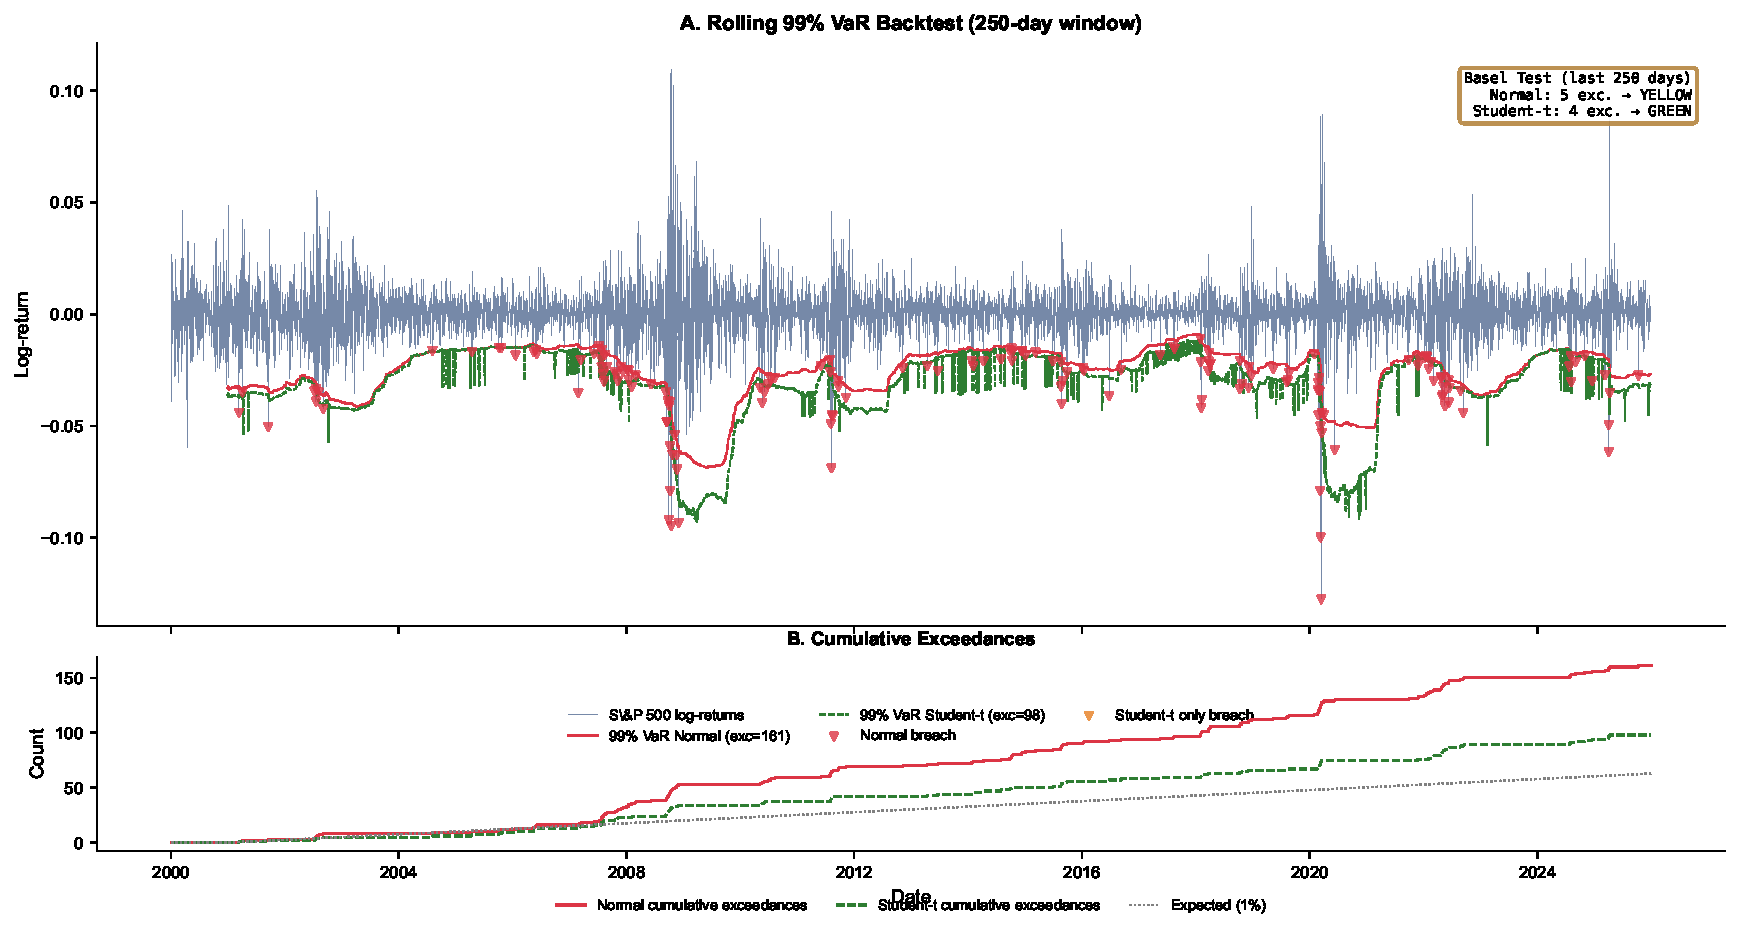
\includegraphics[width=\textwidth]{ch2_var_backtest.pdf}
            {\tiny Backtest: excepțiile marcate cu roșu}
        \end{column}
    \end{columns}
    \quantlet{SFM\_ch2\_risk\_management}{https://github.com/QuantLet/Stat_fin_markets/tree/master/Ch_02/SFM_ch2_risk_management}
    \end{cminipage}
\end{frame}

\begin{frame}{Test 2: Sistemul Basel}
    \begin{cminipage}{0.95\textwidth}
    \begin{alertblock}{Întrebare}
        \begin{itemize}\setlength{\itemsep}{0pt}
            \item În sistemul Basel, 7 excepții pe 250 zile (VaR 1\%) corespund zonei:
        \end{itemize}
    \end{alertblock}

    \begin{block}{Variante de răspuns}
    \begin{itemize}\setlength{\itemsep}{0pt}
        \item \textcolor{MainBlue}{\textbf{(A)}} Verde
        \item \textcolor{MainBlue}{\textbf{(B)}} Galben
        \item \textcolor{MainBlue}{\textbf{(C)}} Roșu
        \item \textcolor{MainBlue}{\textbf{(D)}} Nu este specificat
    \end{itemize}
    \end{block}
    \end{cminipage}
\end{frame}

\begin{frame}{Test 2: Răspuns}
    \begin{cminipage}{0.95\textwidth}
    \begin{columns}[T]
        \begin{column}{0.52\textwidth}
            \begin{exampleblock}{Răspuns: B}
                \begin{itemize}\setlength{\itemsep}{0pt}
                    \item Zona galbenă (5--9 excepții)
                \end{itemize}
            \end{exampleblock}

            \vspace{0.2cm}

            \begin{itemize}\setlength{\itemsep}{0pt}
                \item \textbf{Basel Traffic Light (250 zile):}
            \end{itemize}
            \renewcommand{\arraystretch}{1.2}
            \begin{tabular}{cl}
            \toprule
            \textbf{Excepții} & \textbf{Zona} \\
            \midrule
            0--4 & \textcolor{Forest}{Verde} ($k = 3.0$) \\
            5--9 & \textcolor{Amber}{Galben} ($k \in [3.4, 3.85]$) \\
            $\geq 10$ & \textcolor{Crimson}{Roșu} ($k = 4.0$) \\
            \bottomrule
            \end{tabular}

            \vspace{0.2cm}
            \begin{itemize}\setlength{\itemsep}{0pt}
                \item 7 excepții: zona galben, supraveghere sporită.
            \end{itemize}
        \end{column}
        \begin{column}{0.45\textwidth}
            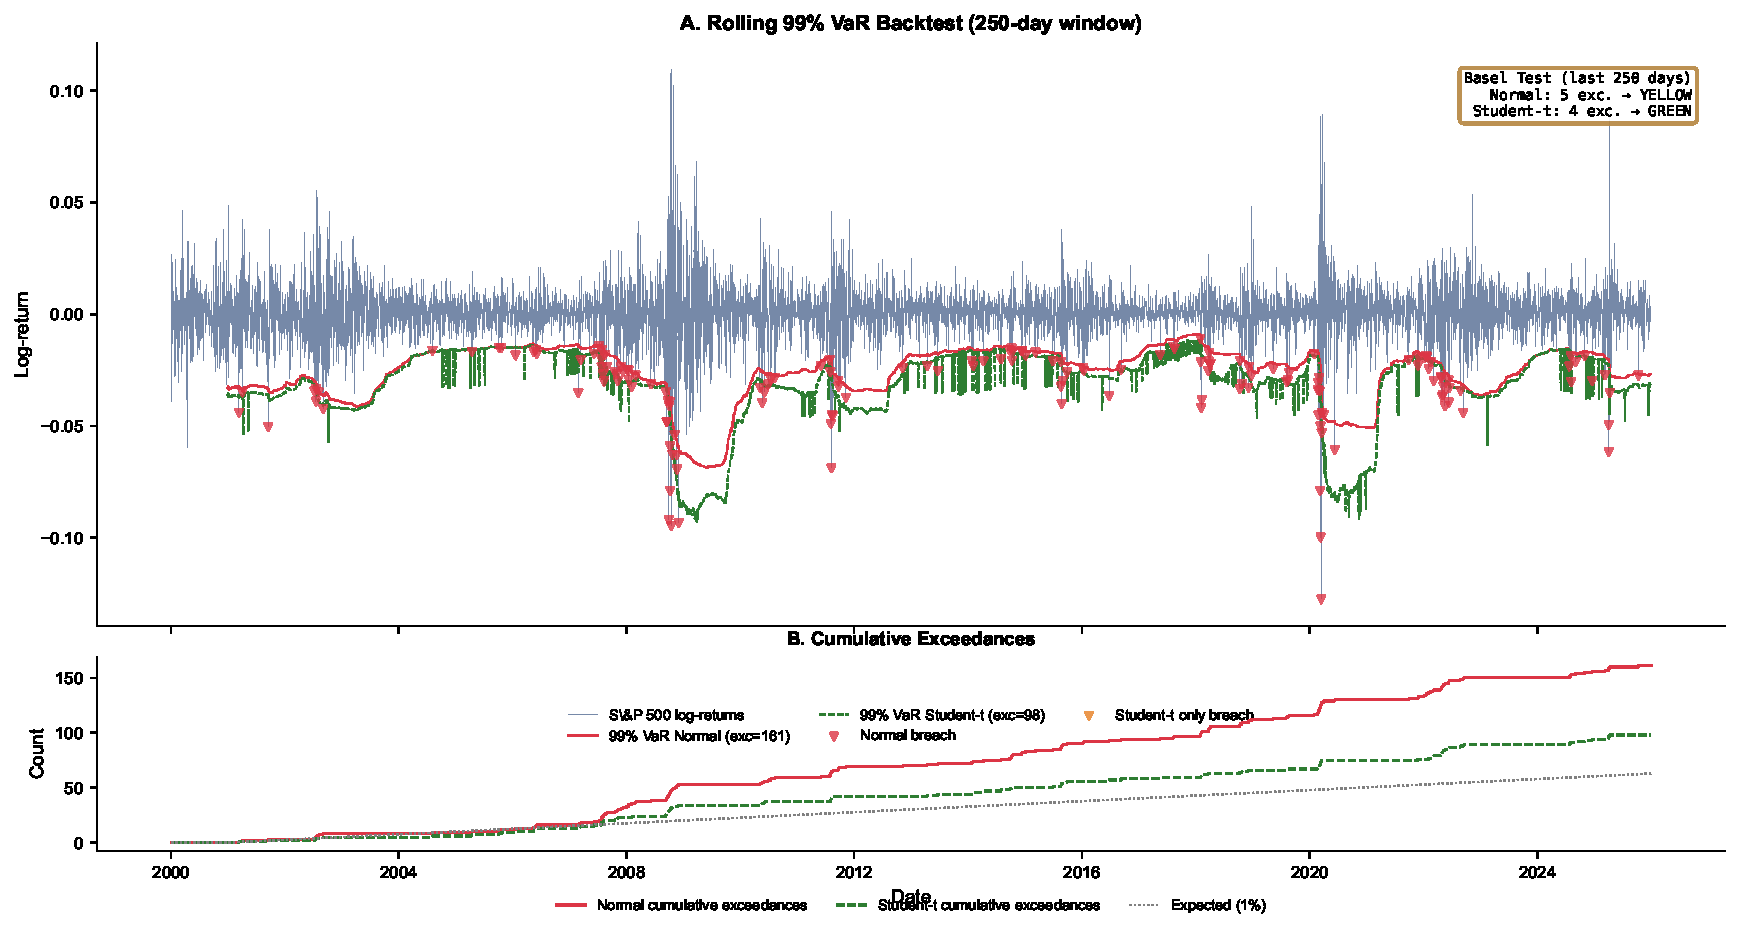
\includegraphics[width=\textwidth]{ch2_var_backtest.pdf}
            {\tiny Basel: multiplicatorul de capital depinde de zona}
        \end{column}
    \end{columns}
    \quantlet{SFM\_ch2\_risk\_management}{https://github.com/QuantLet/Stat_fin_markets/tree/master/Ch_02/SFM_ch2_risk_management}
    \end{cminipage}
\end{frame}

\begin{frame}{Test 3: Persistența GARCH}
    \begin{cminipage}{0.95\textwidth}
    \begin{alertblock}{Întrebare}
        \begin{itemize}\setlength{\itemsep}{0pt}
            \item În GARCH(1,1), $\alpha_1 + \beta_1 = 0.98$ semnifică:
        \end{itemize}
    \end{alertblock}

    \begin{block}{Variante de răspuns}
    \begin{itemize}\setlength{\itemsep}{0pt}
        \item \textcolor{MainBlue}{\textbf{(A)}} Volatilitate scăzută
        \item \textcolor{MainBlue}{\textbf{(B)}} Persistență foarte ridicată a volatilității
        \item \textcolor{MainBlue}{\textbf{(C)}} Modelul este nestaționar
        \item \textcolor{MainBlue}{\textbf{(D)}} Randamentele sunt normale
    \end{itemize}
    \end{block}
    \end{cminipage}
\end{frame}

\begin{frame}{Test 3: Răspuns}
    \begin{cminipage}{0.95\textwidth}
    \begin{columns}[T]
        \begin{column}{0.52\textwidth}
            \begin{exampleblock}{Răspuns: B}
                \begin{itemize}\setlength{\itemsep}{0pt}
                    \item Persistență ridicată --- șocurile se disipează lent
                \end{itemize}
            \end{exampleblock}

            \vspace{0.2cm}

            \begin{itemize}\setlength{\itemsep}{0pt}
                \item \textbf{GARCH(1,1):}
            \end{itemize}
            $$\sigma_t^2 = \omega + \alpha_1 \varepsilon_{t-1}^2 + \beta_1 \sigma_{t-1}^2$$

            \begin{itemize}\setlength{\itemsep}{0pt}
                \item $\alpha_1 + \beta_1 < 1$: staționar \correct
                \item $\alpha_1 + \beta_1 = 1$: IGARCH (memorie infinită)
                \item Persistența $= \alpha_1 + \beta_1 = 0.98$
                \item Timpul de înjumătățire: $\sim 34$ zile
            \end{itemize}
        \end{column}
        \begin{column}{0.45\textwidth}
            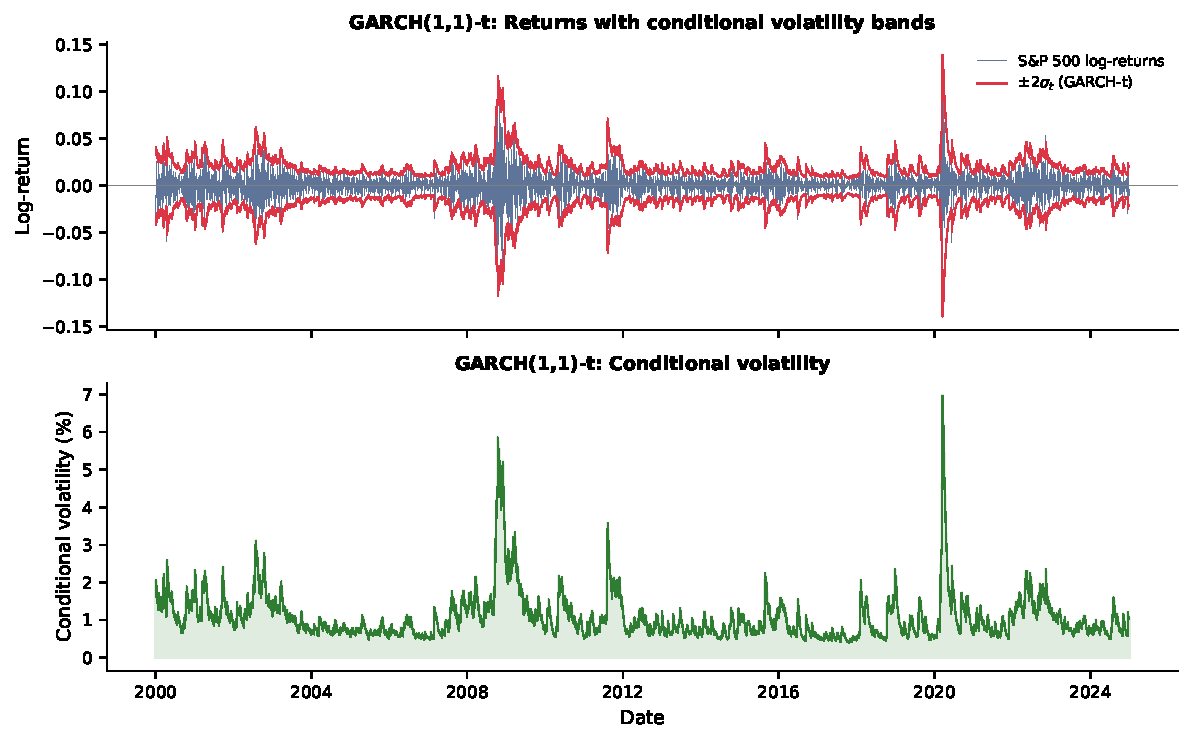
\includegraphics[width=\textwidth]{ch2_garch_t_fit.pdf}
            {\tiny GARCH: volatilitate condiționată dinamică}
        \end{column}
    \end{columns}
    \quantlet{SFM\_ch2\_modern\_extensions}{https://github.com/QuantLet/Stat_fin_markets/tree/master/Ch_02/SFM_ch2_modern_extensions}
    \end{cminipage}
\end{frame}

\begin{frame}{Test 4: Copula Gaussiană}
    \begin{cminipage}{0.95\textwidth}
    \begin{alertblock}{Întrebare}
        \begin{itemize}\setlength{\itemsep}{0pt}
            \item Copula Gaussiană are dependență de coadă $\lambda_L$:
        \end{itemize}
    \end{alertblock}

    \begin{block}{Variante de răspuns}
    \begin{itemize}\setlength{\itemsep}{0pt}
        \item \textcolor{MainBlue}{\textbf{(A)}} $\lambda_L = 1$
        \item \textcolor{MainBlue}{\textbf{(B)}} $\lambda_L = 0.5$
        \item \textcolor{MainBlue}{\textbf{(C)}} $\lambda_L = 0$
        \item \textcolor{MainBlue}{\textbf{(D)}} Depinde de corelația $\rho$
    \end{itemize}
    \end{block}
    \end{cminipage}
\end{frame}

\begin{frame}{Test 4: Răspuns}
    \begin{cminipage}{0.95\textwidth}
    \begin{columns}[T]
        \begin{column}{0.52\textwidth}
            \begin{exampleblock}{Răspuns: C}
                \begin{itemize}\setlength{\itemsep}{0pt}
                    \item $\lambda_L = 0$ (nicio dependență de coadă)
                \end{itemize}
            \end{exampleblock}

            \vspace{0.2cm}

            \begin{itemize}\setlength{\itemsep}{0pt}
                \item \textbf{Dependența de coadă:}
            \end{itemize}
            $$\lambda_L = \lim_{u \to 0^+} P(U_1 \leq u \mid U_2 \leq u)$$

            \begin{itemize}\setlength{\itemsep}{0pt}
                \item Gaussiană: $\lambda_L = 0$ (indiferent de $\rho$) \correct
                \item Student-$t$: $\lambda_L > 0$ (depinde de $\nu, \rho$)
                \item Clayton: $\lambda_L > 0$, $\lambda_U = 0$
                \item $\Rightarrow$ Gaussiana subestimează riscul de crash simultan.
            \end{itemize}
        \end{column}
        \begin{column}{0.45\textwidth}
            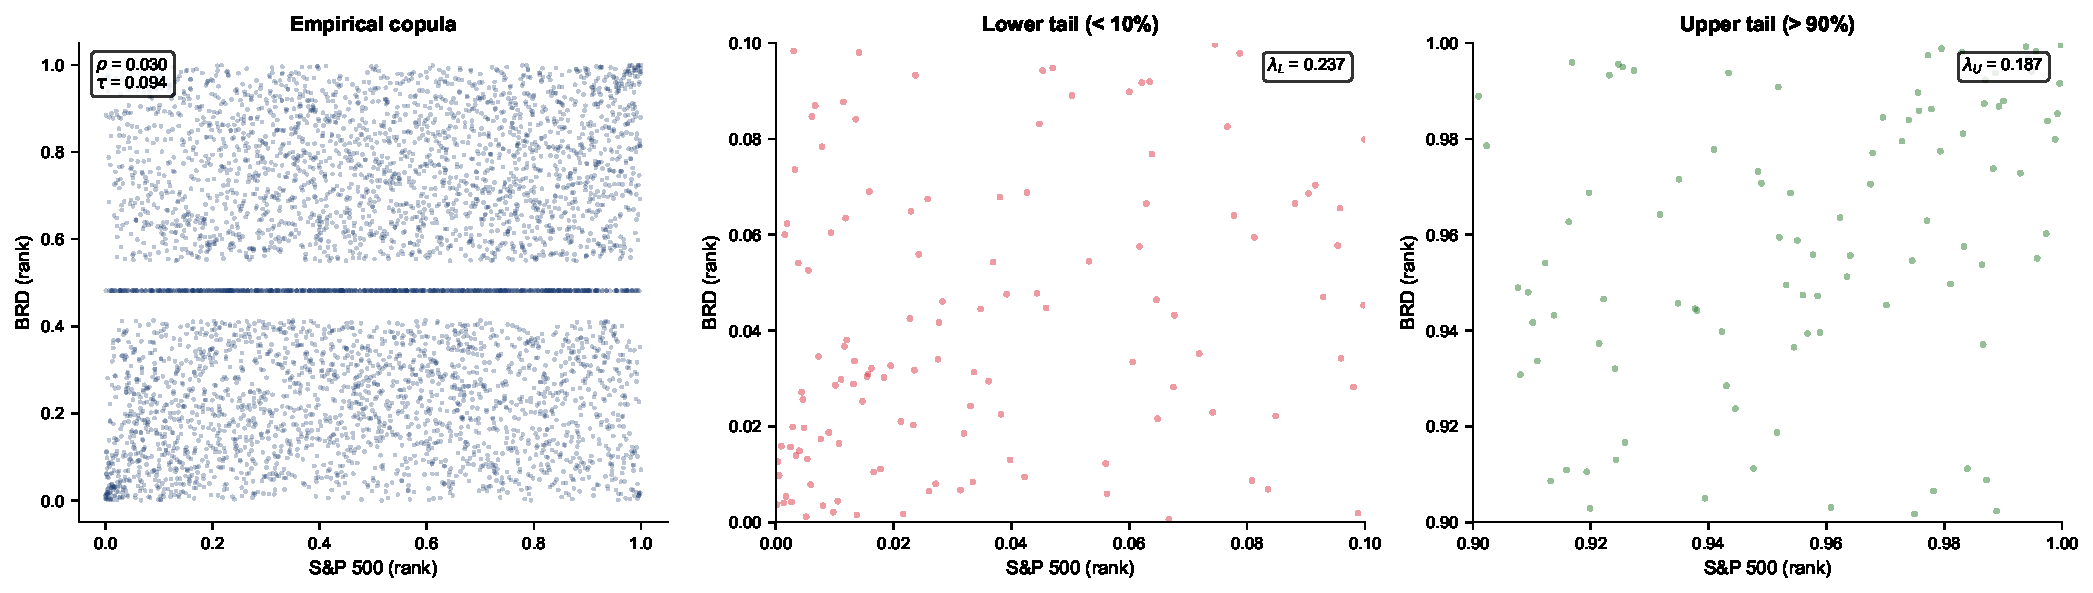
\includegraphics[width=\textwidth]{ch2_cs2c_copula_scatter.pdf}
            {\tiny Copule: Gaussiană vs Student-$t$}
        \end{column}
    \end{columns}
    \quantlet{SFM\_ch2\_modern\_extensions}{https://github.com/QuantLet/Stat_fin_markets/tree/master/Ch_02/SFM_ch2_modern_extensions}
    \end{cminipage}
\end{frame}

\begin{frame}{Test 5: GARCH-$t$ vs VaR Normal}
    \begin{cminipage}{0.95\textwidth}
    \begin{alertblock}{Întrebare}
        \begin{itemize}\setlength{\itemsep}{0pt}
            \item Avantajul principal al GARCH-$t$ față de VaR normal static este:
        \end{itemize}
    \end{alertblock}

    \begin{block}{Variante de răspuns}
    \begin{itemize}\setlength{\itemsep}{0pt}
        \item \textcolor{MainBlue}{\textbf{(A)}} Este mai simplu de implementat
        \item \textcolor{MainBlue}{\textbf{(B)}} Captează și clusteringul volatilității și cozile grele
        \item \textcolor{MainBlue}{\textbf{(C)}} Nu necesită date istorice
        \item \textcolor{MainBlue}{\textbf{(D)}} Dă întotdeauna un VaR mai mic
    \end{itemize}
    \end{block}
    \end{cminipage}
\end{frame}

\begin{frame}{Test 5: Răspuns}
    \begin{cminipage}{0.95\textwidth}
    \begin{columns}[T]
        \begin{column}{0.52\textwidth}
            \begin{exampleblock}{Răspuns: B}
                \begin{itemize}\setlength{\itemsep}{0pt}
                    \item Combinația cozi grele + volatilitate dinamică
                \end{itemize}
            \end{exampleblock}

            \vspace{0.2cm}

            \begin{itemize}\setlength{\itemsep}{0pt}
                \item \textbf{GARCH-$t$ combină:}
                \begin{itemize}\setlength{\itemsep}{0pt}
                    \item Volatilitate condiționată ($\sigma_t$ dinamic)
                    \item Cozi grele (distribuția $t_\nu$)
                    \item VaR se adaptează la regim
                \end{itemize}
            \end{itemize}

            \vspace{0.2cm}
            \begin{itemize}\setlength{\itemsep}{0pt}
                \item Verificare:
                \begin{itemize}\setlength{\itemsep}{0pt}
                    \item A: Mai complex \incorrect
                    \item C: Necesită date \incorrect
                    \item D: VaR poate fi mai mic \textit{sau} mai mare \incorrect
                \end{itemize}
            \end{itemize}
        \end{column}
        \begin{column}{0.45\textwidth}
            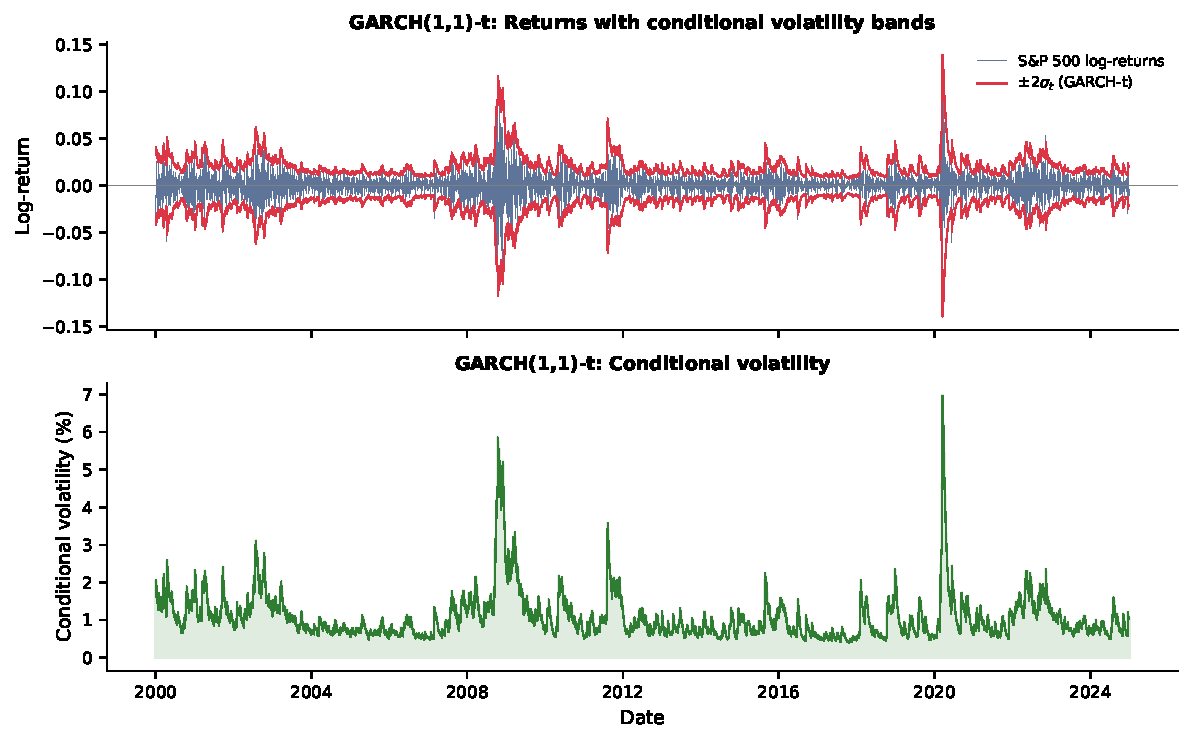
\includegraphics[width=\textwidth]{ch2_garch_t_fit.pdf}
            {\tiny GARCH-$t$: se adaptează la volatilitate}
        \end{column}
    \end{columns}
    \quantlet{SFM\_ch2\_modern\_extensions}{https://github.com/QuantLet/Stat_fin_markets/tree/master/Ch_02/SFM_ch2_modern_extensions}
    \end{cminipage}
\end{frame}

\begin{frame}{Test 6: Fereastră rolling}
    \begin{cminipage}{0.95\textwidth}
    \begin{alertblock}{Întrebare}
        \begin{itemize}\setlength{\itemsep}{0pt}
            \item O fereastră rolling de 250 zile vs 500 zile pentru estimarea VaR:
        \end{itemize}
    \end{alertblock}

    \begin{block}{Variante de răspuns}
    \begin{itemize}\setlength{\itemsep}{0pt}
        \item \textcolor{MainBlue}{\textbf{(A)}} 250 zile reacționează mai rapid la schimbări de regim
        \item \textcolor{MainBlue}{\textbf{(B)}} 500 zile reacționează mai rapid
        \item \textcolor{MainBlue}{\textbf{(C)}} Nu există diferență
        \item \textcolor{MainBlue}{\textbf{(D)}} 250 zile este întotdeauna mai bun
    \end{itemize}
    \end{block}
    \end{cminipage}
\end{frame}

\begin{frame}{Test 6: Răspuns}
    \begin{cminipage}{0.95\textwidth}
    \begin{columns}[T]
        \begin{column}{0.52\textwidth}
            \begin{exampleblock}{Răspuns: A}
                \begin{itemize}\setlength{\itemsep}{0pt}
                    \item Fereastră mai scurtă $=$ reacție mai rapidă
                \end{itemize}
            \end{exampleblock}

            \vspace{0.2cm}

            \begin{itemize}\setlength{\itemsep}{0pt}
                \item \textbf{Compromisul fereastră rolling:}
                \begin{itemize}\setlength{\itemsep}{0pt}
                    \item Fereastră scurtă: \textcolor{Forest}{reactivitate}, \textcolor{Crimson}{instabilitate}
                    \item Fereastră lungă: \textcolor{Forest}{stabilitate}, \textcolor{Crimson}{lentoare}
                \end{itemize}
            \end{itemize}

            \vspace{0.2cm}
            \begin{itemize}\setlength{\itemsep}{0pt}
                \item Verificare:
                \begin{itemize}\setlength{\itemsep}{0pt}
                    \item B: Invers \incorrect
                    \item C: Diferă semnificativ \incorrect
                    \item D: Depinde de context \incorrect
                \end{itemize}
            \end{itemize}
        \end{column}
        \begin{column}{0.45\textwidth}
            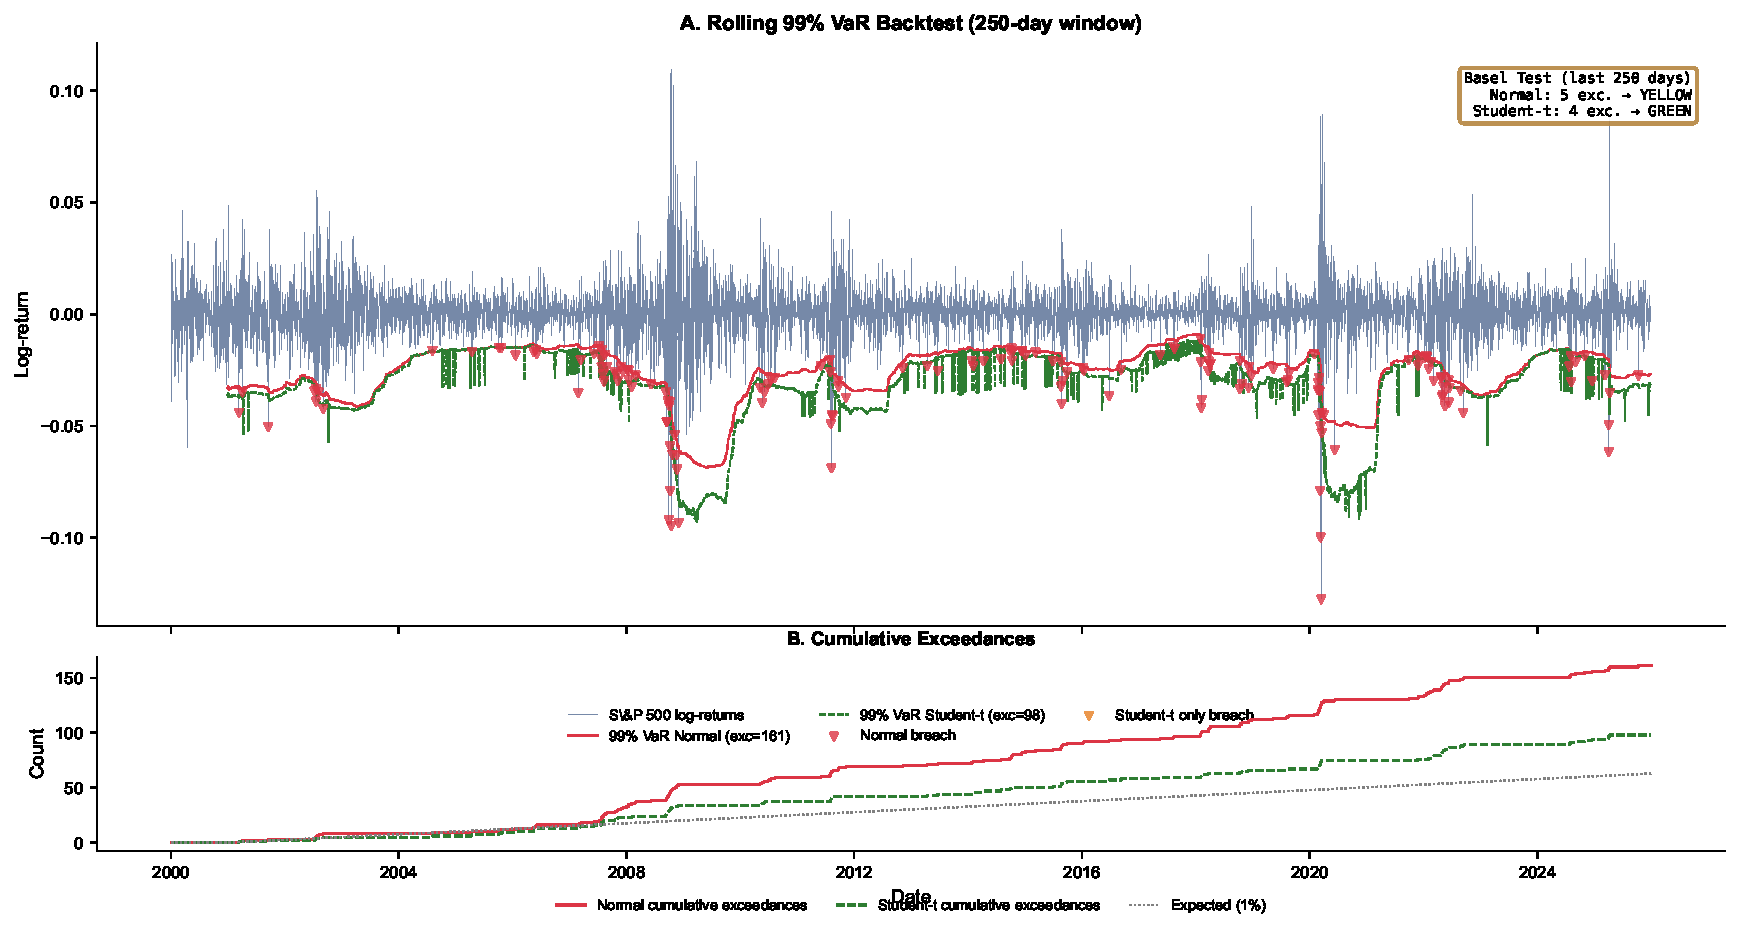
\includegraphics[width=\textwidth]{ch2_var_backtest.pdf}
            {\tiny Rolling VaR: fereastră 250 zile}
        \end{column}
    \end{columns}
    \quantlet{SFM\_ch2\_risk\_management}{https://github.com/QuantLet/Stat_fin_markets/tree/master/Ch_02/SFM_ch2_risk_management}
    \end{cminipage}
\end{frame}

\begin{frame}{Test 7: Testul Christoffersen}
    \begin{cminipage}{0.95\textwidth}
    \begin{alertblock}{Întrebare}
        \begin{itemize}\setlength{\itemsep}{0pt}
            \item Testul Christoffersen adaugă față de testul Kupiec:
        \end{itemize}
    \end{alertblock}

    \begin{block}{Variante de răspuns}
    \begin{itemize}\setlength{\itemsep}{0pt}
        \item \textcolor{MainBlue}{\textbf{(A)}} Testul de normalitate a reziduurilor
        \item \textcolor{MainBlue}{\textbf{(B)}} Testul de independență al excepțiilor
        \item \textcolor{MainBlue}{\textbf{(C)}} Testul de staționaritate
        \item \textcolor{MainBlue}{\textbf{(D)}} Testul de heteroscedasticitate
    \end{itemize}
    \end{block}
    \end{cminipage}
\end{frame}

\begin{frame}{Test 7: Răspuns}
    \begin{cminipage}{0.95\textwidth}
    \begin{columns}[T]
        \begin{column}{0.52\textwidth}
            \begin{exampleblock}{Răspuns: B}
                \begin{itemize}\setlength{\itemsep}{0pt}
                    \item Christoffersen testează și \textbf{independența} excepțiilor
                \end{itemize}
            \end{exampleblock}

            \vspace{0.2cm}

            \begin{itemize}\setlength{\itemsep}{0pt}
                \item \textbf{Kupiec vs Christoffersen:}
                \begin{itemize}\setlength{\itemsep}{0pt}
                    \item Kupiec (POF): doar frecvența $\hat{p} \approx \alpha$
                    \item Christoffersen (CC): frecvența + independența
                \end{itemize}
            \end{itemize}

            \vspace{0.2cm}
            \begin{itemize}\setlength{\itemsep}{0pt}
                \item $\text{LR}_{\text{CC}} = \text{LR}_{\text{POF}} + \text{LR}_{\text{IND}} \sim \chi^2(2)$
                \item Excepțiile grupate $\Rightarrow$ model inadecvat.
            \end{itemize}
        \end{column}
        \begin{column}{0.45\textwidth}
            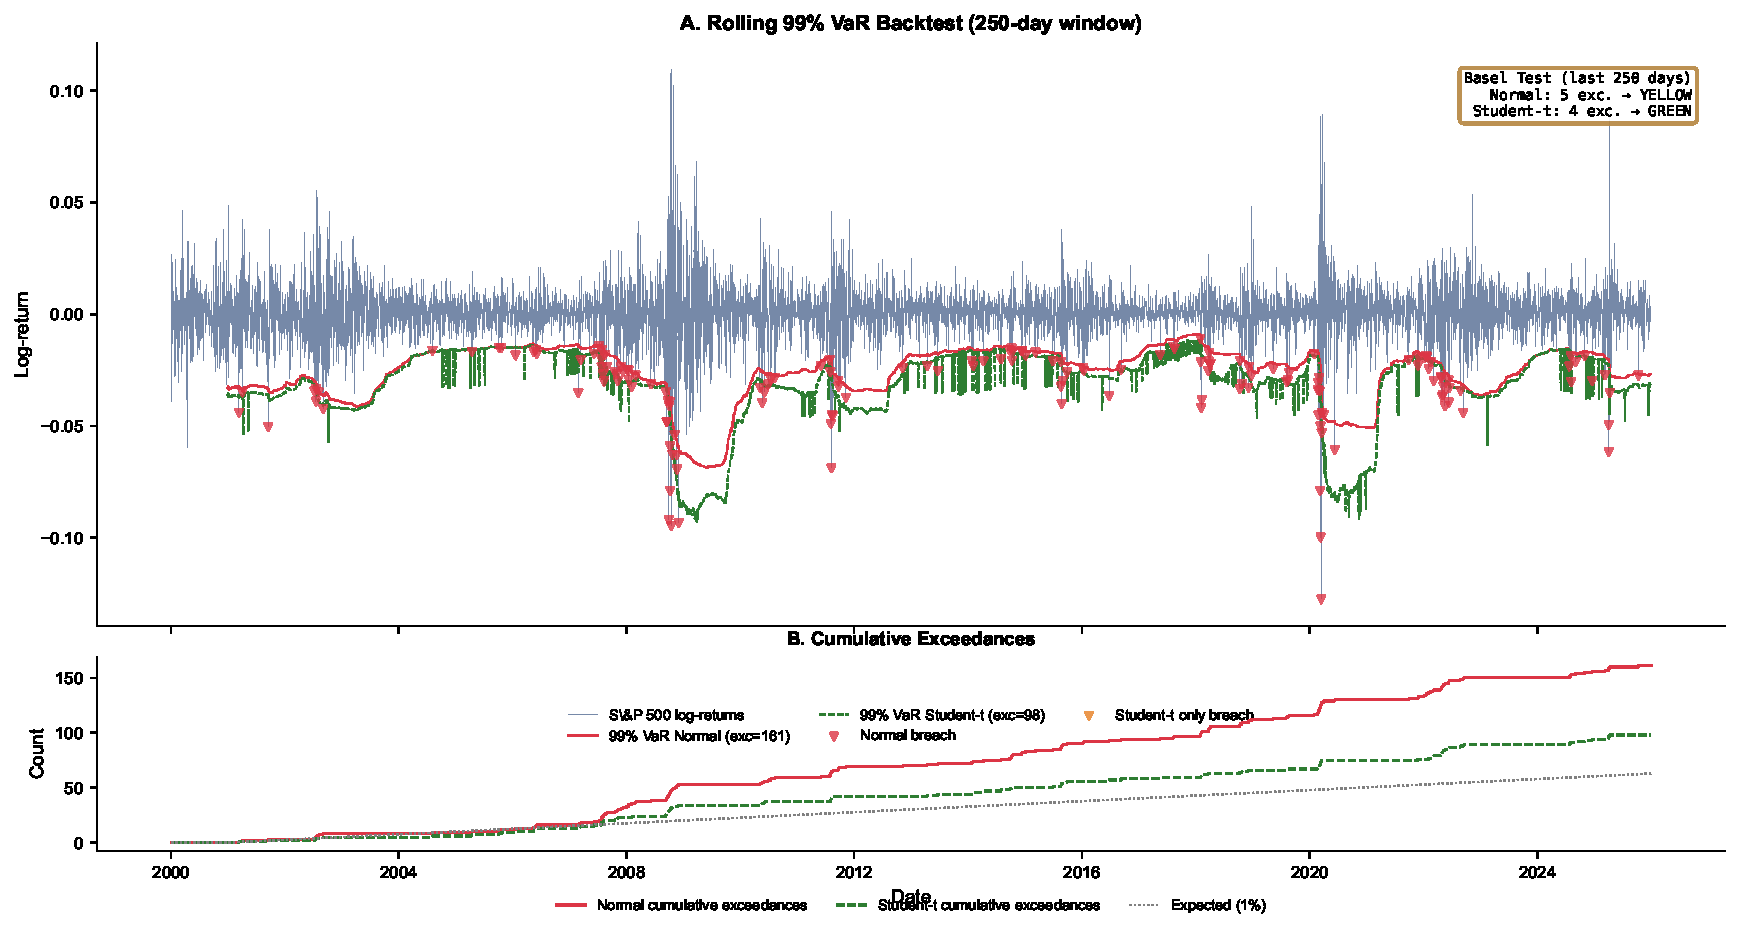
\includegraphics[width=\textwidth]{ch2_var_backtest.pdf}
            {\tiny Excepțiile grupate: modelul nu captează clustering}
        \end{column}
    \end{columns}
    \quantlet{SFM\_ch2\_risk\_management}{https://github.com/QuantLet/Stat_fin_markets/tree/master/Ch_02/SFM_ch2_risk_management}
    \end{cminipage}
\end{frame}

\begin{frame}{Test 8: Sub-aditivitatea VaR}
    \begin{cminipage}{0.95\textwidth}
    \begin{alertblock}{Întrebare}
        \begin{itemize}\setlength{\itemsep}{0pt}
            \item VaR nu este subaditivă. Aceasta înseamnă că:
        \end{itemize}
    \end{alertblock}

    \begin{block}{Variante de răspuns}
    \begin{itemize}\setlength{\itemsep}{0pt}
        \item \textcolor{MainBlue}{\textbf{(A)}} $\text{VaR}(A+B) \leq \text{VaR}(A) + \text{VaR}(B)$ întotdeauna
        \item \textcolor{MainBlue}{\textbf{(B)}} Este posibil ca $\text{VaR}(A+B) > \text{VaR}(A) + \text{VaR}(B)$
        \item \textcolor{MainBlue}{\textbf{(C)}} $\text{VaR}(A+B) = \text{VaR}(A) + \text{VaR}(B)$ întotdeauna
        \item \textcolor{MainBlue}{\textbf{(D)}} VaR este întotdeauna zero pentru portofolii diversificate
    \end{itemize}
    \end{block}
    \end{cminipage}
\end{frame}

\begin{frame}{Test 8: Răspuns}
    \begin{cminipage}{0.95\textwidth}
    \begin{columns}[T]
        \begin{column}{0.52\textwidth}
            \begin{exampleblock}{Răspuns: B}
                \begin{itemize}\setlength{\itemsep}{0pt}
                    \item Diversificarea poate \textit{crește} VaR-ul
                \end{itemize}
            \end{exampleblock}

            \vspace{0.2cm}

            \begin{itemize}\setlength{\itemsep}{0pt}
                \item \textbf{Consecințe:}
                \begin{itemize}\setlength{\itemsep}{0pt}
                    \item VaR nu recompensează diversificarea
                    \item ES este subaditivă \correct
                    \item Basel III/IV preferă ES
                \end{itemize}
            \end{itemize}

            \vspace{0.2cm}
            \begin{itemize}\setlength{\itemsep}{0pt}
                \item VaR nu satisface axiomele Artzner (1999) $\Rightarrow$ \textbf{nu este coerentă}.
                \item ES satisface toate axiomele $\Rightarrow$ coerentă.
            \end{itemize}
        \end{column}
        \begin{column}{0.45\textwidth}
            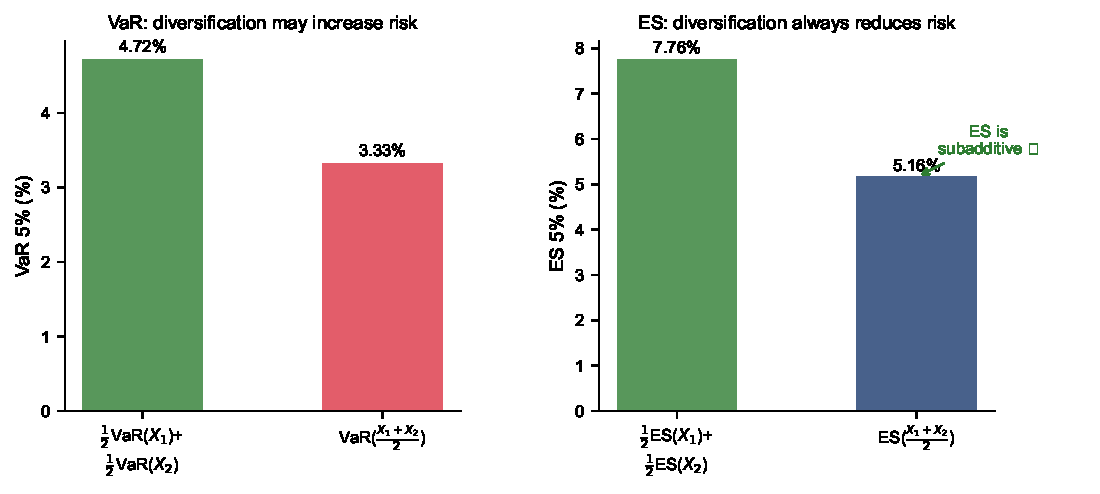
\includegraphics[width=\textwidth]{ch2_var_subadditivity.pdf}
            {\tiny VaR: contra-exemplu sub-aditivitate}
        \end{column}
    \end{columns}
    \quantlet{SFM\_ch2\_risk\_management}{https://github.com/QuantLet/Stat_fin_markets/tree/master/Ch_02/SFM_ch2_risk_management}
    \end{cminipage}
\end{frame}

\begin{frame}{Test 9: Backtesting ES}
    \begin{cminipage}{0.95\textwidth}
    \begin{alertblock}{Întrebare}
        \begin{itemize}\setlength{\itemsep}{0pt}
            \item Diferența principală dintre backtesting VaR și backtesting ES este:
        \end{itemize}
    \end{alertblock}

    \begin{block}{Variante de răspuns}
    \begin{itemize}\setlength{\itemsep}{0pt}
        \item \textcolor{MainBlue}{\textbf{(A)}} ES nu poate fi testat niciodată
        \item \textcolor{MainBlue}{\textbf{(B)}} ES necesită \textbf{magnitudinea} pierderilor, nu doar frecvența
        \item \textcolor{MainBlue}{\textbf{(C)}} Nu există diferență
        \item \textcolor{MainBlue}{\textbf{(D)}} VaR backtesting este mai complex decât ES
    \end{itemize}
    \end{block}
    \end{cminipage}
\end{frame}

\begin{frame}{Test 9: Răspuns}
    \begin{cminipage}{0.95\textwidth}
    \begin{columns}[T]
        \begin{column}{0.52\textwidth}
            \begin{exampleblock}{Răspuns: B}
                \begin{itemize}\setlength{\itemsep}{0pt}
                    \item ES necesită evaluarea \textbf{cât de mare} a fost pierderea
                \end{itemize}
            \end{exampleblock}

            \vspace{0.2cm}

            \begin{itemize}\setlength{\itemsep}{0pt}
                \item \textbf{Comparație:}
                \begin{itemize}\setlength{\itemsep}{0pt}
                    \item VaR backtest: a fost depășit? (da/nu)
                    \item ES backtest: cât de mult a fost depășit?
                \end{itemize}
            \end{itemize}

            \vspace{0.2cm}
            \begin{itemize}\setlength{\itemsep}{0pt}
                \item Verificare:
                \begin{itemize}\setlength{\itemsep}{0pt}
                    \item A: ES poate fi testat (Acerbi \& Szekely, 2014) \incorrect
                    \item C: Diferă fundamental \incorrect
                    \item D: ES este mai greu de testat \incorrect
                \end{itemize}
            \end{itemize}
        \end{column}
        \begin{column}{0.45\textwidth}
            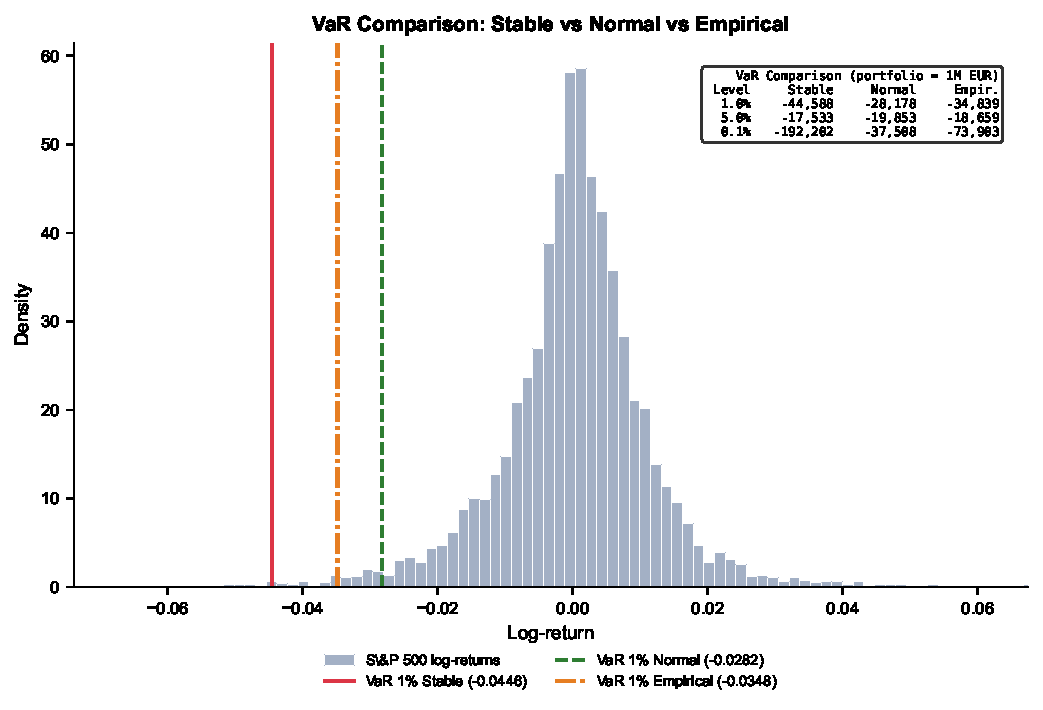
\includegraphics[width=\textwidth]{ch2_var_comparison.pdf}
            {\tiny ES: media pierderilor dincolo de VaR}
        \end{column}
    \end{columns}
    \quantlet{SFM\_ch2\_risk\_management}{https://github.com/QuantLet/Stat_fin_markets/tree/master/Ch_02/SFM_ch2_risk_management}
    \end{cminipage}
\end{frame}

\begin{frame}{Test 10: Parametrii GARCH}
    \begin{cminipage}{0.95\textwidth}
    \begin{alertblock}{Întrebare}
        \begin{itemize}\setlength{\itemsep}{0pt}
            \item În GARCH(1,1), $\alpha_1$ mare vs $\beta_1$ mare semnifică:
        \end{itemize}
    \end{alertblock}

    \begin{block}{Variante de răspuns}
    \begin{itemize}\setlength{\itemsep}{0pt}
        \item \textcolor{MainBlue}{\textbf{(A)}} $\alpha_1$: reacție rapidă la șocuri; $\beta_1$: memorie lungă
        \item \textcolor{MainBlue}{\textbf{(B)}} $\alpha_1$: memorie lungă; $\beta_1$: reacție rapidă
        \item \textcolor{MainBlue}{\textbf{(C)}} Ambii au același efect
        \item \textcolor{MainBlue}{\textbf{(D)}} Niciun efect asupra volatilității
    \end{itemize}
    \end{block}
    \end{cminipage}
\end{frame}

\begin{frame}{Test 10: Răspuns}
    \begin{cminipage}{0.95\textwidth}
    \begin{columns}[T]
        \begin{column}{0.52\textwidth}
            \begin{exampleblock}{Răspuns: A}
                \begin{itemize}\setlength{\itemsep}{0pt}
                    \item $\alpha_1$ = reactivitate, $\beta_1$ = persistență
                \end{itemize}
            \end{exampleblock}

            \vspace{0.2cm}

            \begin{itemize}\setlength{\itemsep}{0pt}
                \item \textbf{GARCH(1,1):}
            \end{itemize}
            $$\sigma_t^2 = \omega + \underbrace{\alpha_1 \varepsilon_{t-1}^2}_{\text{reacție la șoc}} + \underbrace{\beta_1 \sigma_{t-1}^2}_{\text{inerție}}$$

            \begin{itemize}\setlength{\itemsep}{0pt}
                \item Valori tipice pe acțiuni:
                \begin{itemize}\setlength{\itemsep}{0pt}
                    \item $\hat{\alpha}_1 \approx 0.05$--$0.10$ (reacție moderată)
                    \item $\hat{\beta}_1 \approx 0.85$--$0.95$ (persistență ridicată)
                    \item $\hat{\alpha}_1 + \hat{\beta}_1 \approx 0.95$--$0.99$
                \end{itemize}
            \end{itemize}
        \end{column}
        \begin{column}{0.45\textwidth}
            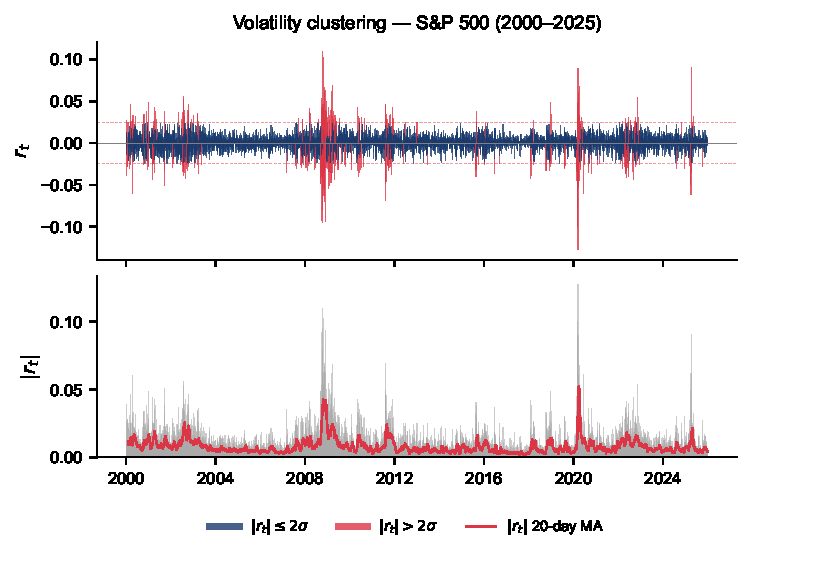
\includegraphics[width=\textwidth]{ch2_volatility_clustering.pdf}
            {\tiny GARCH: clustering-ul volatilității}
        \end{column}
    \end{columns}
    \quantlet{SFM\_ch2\_modern\_extensions}{https://github.com/QuantLet/Stat_fin_markets/tree/master/Ch_02/SFM_ch2_modern_extensions}
    \end{cminipage}
\end{frame}

%=============================================================================
% PART 2: TRUE/FALSE QUESTIONS
%=============================================================================
\section{Întrebări Adevărat/Fals}

\begin{frame}{Adevărat sau Fals? --- Întrebări}
    \begin{cminipage}{0.95\textwidth}
    \begin{itemize}\setlength{\itemsep}{0pt}
        \item \textbf{Răspundeți cu Adevărat (A) sau Fals (F):}
    \end{itemize}
    \vspace{0.3cm}
    \begin{enumerate}\setlength{\itemsep}{0pt}
        \item AIC și BIC pot selecta modele diferite, iar ambele pot fi ``corecte''.
        \item Testul Kupiec detectează atât frecvența cât și gruparea excepțiilor VaR.
        \item Un model VaR cu 0 excepții pe 250 zile este modelul ideal.
        \item GARCH(1,1) cu $\alpha_1 + \beta_1 = 1$ se numește IGARCH.
        \item Copula Gaussiană subestimează riscul de crash simultan.
        \item Backtesting-ul VaR elimină complet riscul de model.
    \end{enumerate}
    \end{cminipage}
\end{frame}

\begin{frame}{Adevărat sau Fals? --- Răspunsuri}
    \begin{cminipage}{0.95\textwidth}
    \begin{columns}[T]
        \begin{column}{0.55\textwidth}
            \small
            \begin{enumerate}\setlength{\itemsep}{0pt}
                \item \textcolor{Forest}{\textbf{ADEVĂRAT}}: AIC: predicție optimă; BIC: model adevărat
                \vspace{0.1cm}
                \item \textcolor{Crimson}{\textbf{FALS}}: Kupiec testează doar \textit{frecvența}; Christoffersen testează și gruparea
                \vspace{0.1cm}
                \item \textcolor{Crimson}{\textbf{FALS}}: 0 excepții $\Rightarrow$ model prea conservator, capital excesiv
                \vspace{0.1cm}
                \item \textcolor{Forest}{\textbf{ADEVĂRAT}}: IGARCH = Integrated GARCH, persistență unitară
                \vspace{0.1cm}
                \item \textcolor{Forest}{\textbf{ADEVĂRAT}}: $\lambda_L = 0$ pentru Gaussiană, $>0$ în realitate
                \vspace{0.1cm}
                \item \textcolor{Crimson}{\textbf{FALS}}: Backtesting validează \textit{din trecut}; nu garantează viitorul
            \end{enumerate}
        \end{column}
        \begin{column}{0.42\textwidth}
            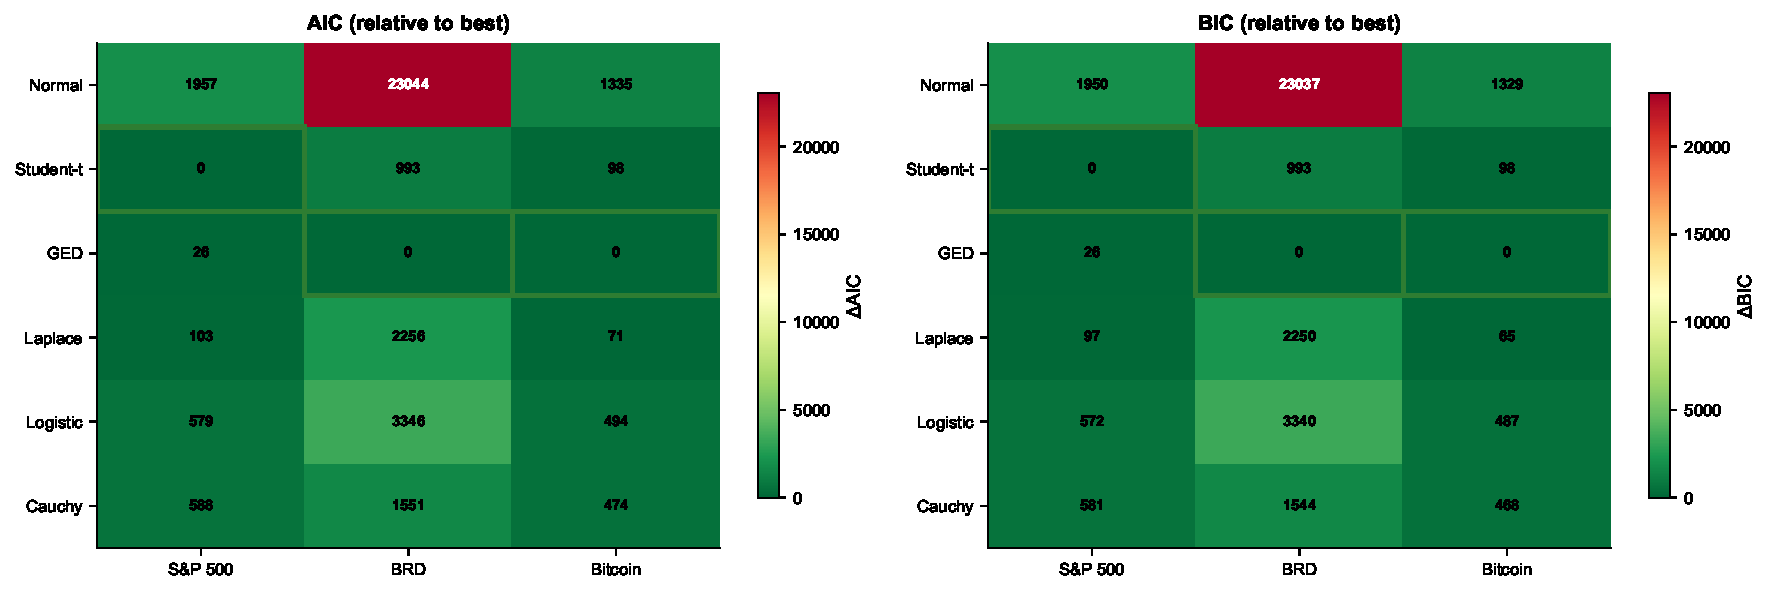
\includegraphics[width=\textwidth]{ch2_cs2c_model_selection_heatmap.pdf}
            {\tiny Selecția modelului variază pe active}
        \end{column}
    \end{columns}
    \quantlet{SFM\_ch2\_case\_study\_2c}{https://github.com/QuantLet/Stat_fin_markets/tree/master/Ch_02/SFM_ch2_case_study_2c}
    \end{cminipage}
\end{frame}

%=============================================================================
% PART 3: CALCULATION EXERCISES
%=============================================================================
\section{Exerciții de Calcul}

\begin{frame}{Exercițiul 1: AIC/BIC pentru 4 distribuții}
    \begin{cminipage}{0.95\textwidth}
    \begin{itemize}\setlength{\itemsep}{0pt}
        \item \textbf{Problemă:} Pe $n = 2000$ randamente, ajustăm 4 distribuții:
    \end{itemize}

    \renewcommand{\arraystretch}{1.2}
    \begin{center}
    \begin{tabular}{lccc}
    \toprule
    \textbf{Model} & $k$ & $\ell$ & \\
    \midrule
    Normal & 2 & 6421 & \\
    Student-$t$ & 3 & 6487 & \\
    Skew-$t$ & 4 & 6504 & \\
    GED & 3 & 6511 & \\
    \bottomrule
    \end{tabular}
    \end{center}

    \begin{itemize}\setlength{\itemsep}{0pt}
        \item Calculați AIC, BIC, și efectuați testul LR: Normal $\subset$ Student-$t$ și Student-$t$ $\subset$ Skew-$t$.
    \end{itemize}
    \end{cminipage}
\end{frame}

\begin{frame}{Exercițiul 1: Soluție}
    \begin{cminipage}{0.95\textwidth}
    \begin{columns}[T]
        \begin{column}{0.52\textwidth}
            \renewcommand{\arraystretch}{1.2}
            \begin{tabular}{lccc}
            \toprule
            \textbf{Model} & \textbf{AIC} & \textbf{BIC} & \textbf{Rang} \\
            \midrule
            Normal & $-12838$ & $-12827$ & 4 \\
            Student-$t$ & $-12968$ & $-12951$ & 3 \\
            Skew-$t$ & $-13000$ & $-12978$ & 2 \\
            GED & $-13016$ & $-12999$ & \textbf{1} \\
            \bottomrule
            \end{tabular}

            \vspace{0.2cm}
            \begin{itemize}\setlength{\itemsep}{0pt}
                \item \textbf{Testul LR:}
                \item Normal vs $t$: $\text{LR} = 2(6487 - 6421) = 132$
                \item $\gg \chi^2_{0.01}(1) = 6.63$ $\Rightarrow$ \textcolor{Crimson}{Respingem} distribuția normală
                \item $t$ vs Skew-$t$: $\text{LR} = 2(6504 - 6487) = 34$
                \item $\Rightarrow$ \textcolor{Crimson}{Respingem} simetria
            \end{itemize}
        \end{column}
        \begin{column}{0.45\textwidth}
            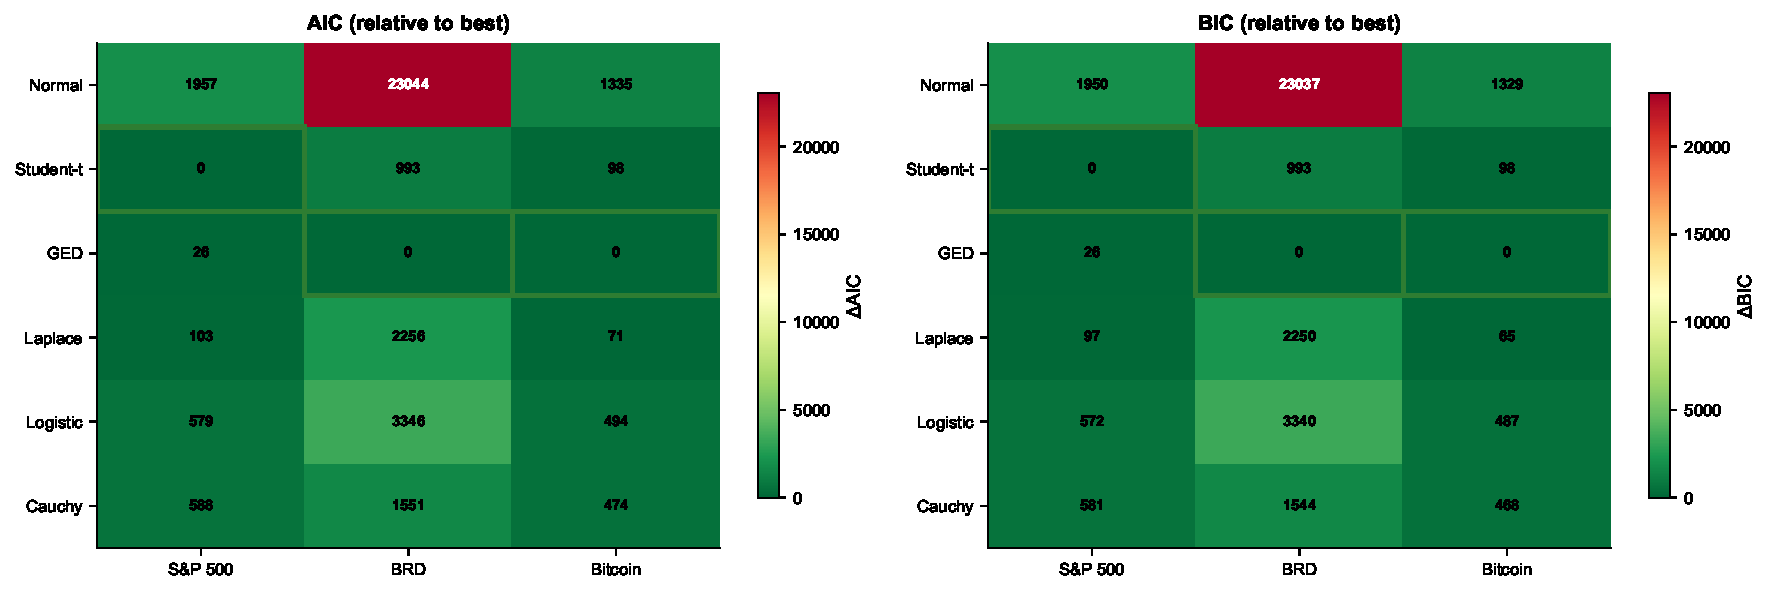
\includegraphics[width=\textwidth]{ch2_cs2c_model_selection_heatmap.pdf}
            {\tiny Heatmap: AIC relativ pe active}
        \end{column}
    \end{columns}
    \quantlet{SFM\_ch2\_case\_study\_2c}{https://github.com/QuantLet/Stat_fin_markets/tree/master/Ch_02/SFM_ch2_case_study_2c}
    \end{cminipage}
\end{frame}

\begin{frame}{Exercițiul 2: Testul Kupiec}
    \begin{cminipage}{0.95\textwidth}
    \begin{itemize}\setlength{\itemsep}{0pt}
        \item \textbf{Problemă:} VaR 1\% testat pe $T = 500$ zile. Analizați $x = 4$, $x = 6$, $x = 12$ excepții.
    \end{itemize}

    \begin{itemize}\setlength{\itemsep}{0pt}
        \item Calculați:
    \end{itemize}
    \begin{enumerate}\setlength{\itemsep}{0pt}
        \item Statistica LR Kupiec pentru fiecare scenariu
        \item Decizia la nivel de semnificație 1\%
        \item Zona Basel (normalizată la 250 zile)
    \end{enumerate}
    \end{cminipage}
\end{frame}

\begin{frame}{Exercițiul 2: Soluție}
    \begin{cminipage}{0.95\textwidth}
    \begin{columns}[T]
        \begin{column}{0.52\textwidth}
            \begin{itemize}\setlength{\itemsep}{0pt}
                \item $\text{LR} = -2\ln\frac{\alpha^x(1-\alpha)^{T-x}}{\hat{p}^x(1-\hat{p})^{T-x}}$, \; $\hat{p} = x/T$
                \item Așteptat: $T\alpha = 5$ excepții.
            \end{itemize}

            \vspace{0.2cm}
            \renewcommand{\arraystretch}{1.2}
            \begin{tabular}{cccc}
            \toprule
            $x$ & $\hat{p}$ & LR & \textbf{Decizie} \\
            \midrule
            4 & 0.80\% & 0.25 & \textcolor{Forest}{Acceptat} \\
            6 & 1.20\% & 0.18 & \textcolor{Forest}{Acceptat} \\
            12 & 2.40\% & 7.14 & \textcolor{Crimson}{Respins} \\
            \bottomrule
            \end{tabular}

            \vspace{0.2cm}
            \begin{itemize}\setlength{\itemsep}{0pt}
                \item \textbf{Basel (250 zile):}
                \begin{itemize}\setlength{\itemsep}{0pt}
                    \item $x=4$: 2 exc/250 $\Rightarrow$ \textcolor{Forest}{Verde}
                    \item $x=6$: 3 exc/250 $\Rightarrow$ \textcolor{Forest}{Verde}
                    \item $x=12$: 6 exc/250 $\Rightarrow$ \textcolor{Amber}{Galben}
                \end{itemize}
            \end{itemize}
        \end{column}
        \begin{column}{0.45\textwidth}
            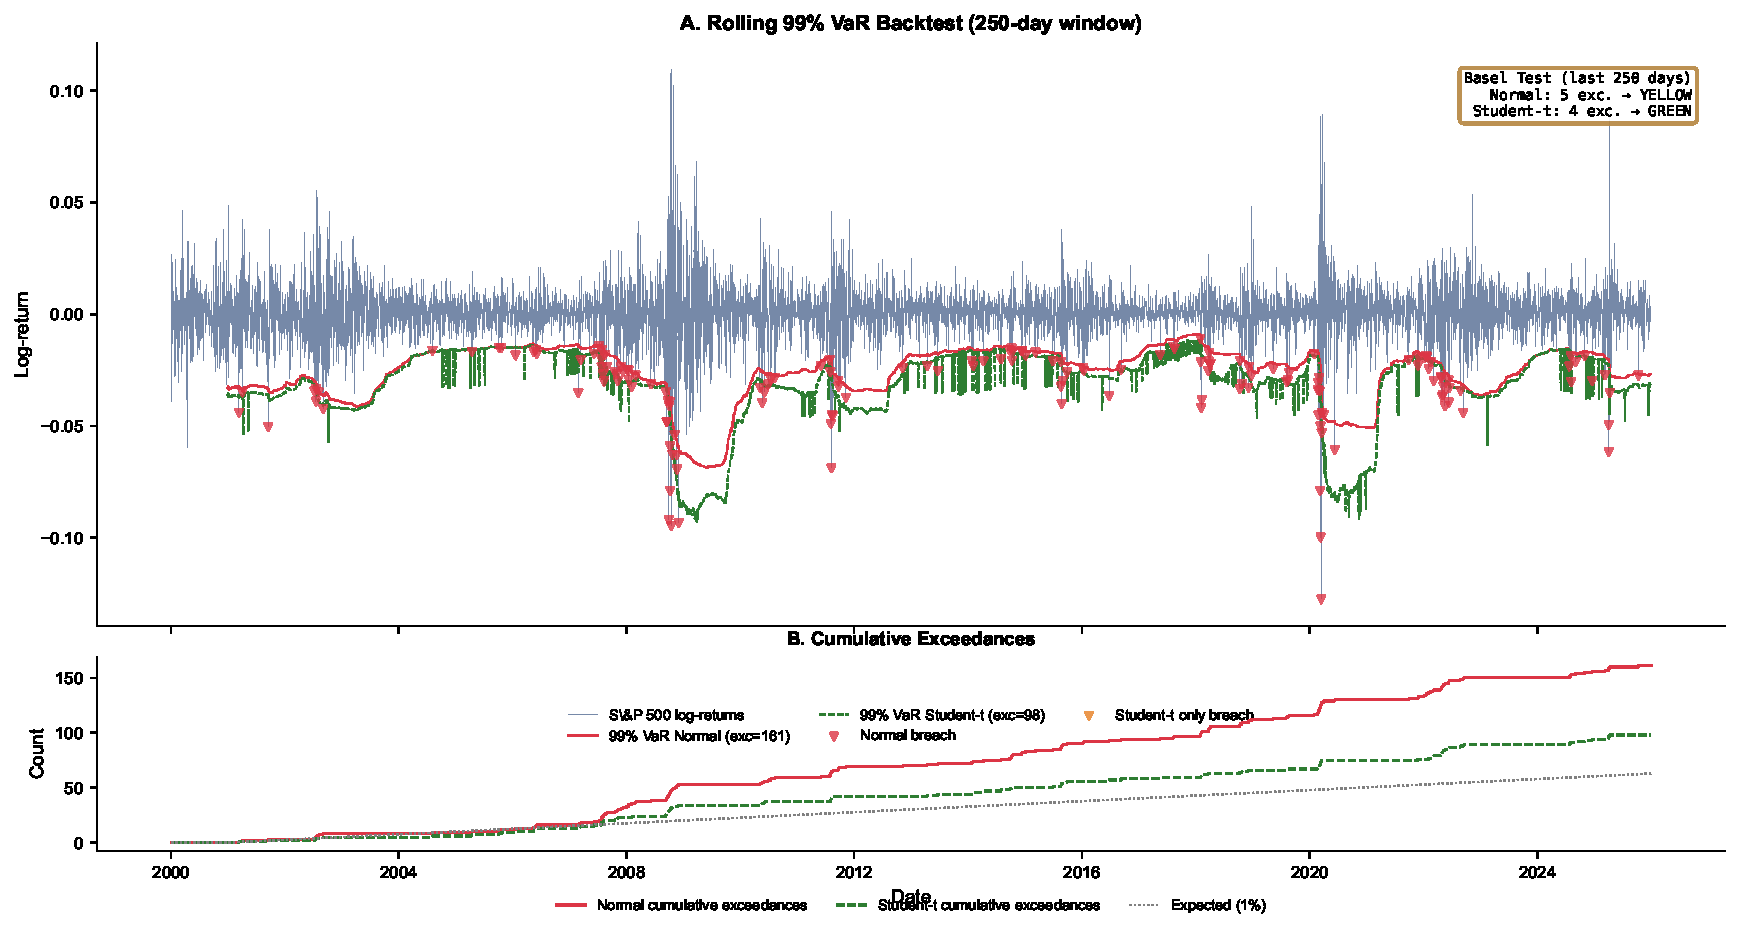
\includegraphics[width=\textwidth]{ch2_var_backtest.pdf}
            {\tiny Backtest VaR: excepții vs randamente}
        \end{column}
    \end{columns}
    \quantlet{SFM\_ch2\_risk\_management}{https://github.com/QuantLet/Stat_fin_markets/tree/master/Ch_02/SFM_ch2_risk_management}
    \end{cminipage}
\end{frame}

\begin{frame}{Exercițiul 3: VaR condiționat GARCH-$t$}
    \begin{cminipage}{0.95\textwidth}
    \begin{itemize}\setlength{\itemsep}{0pt}
        \item \textbf{Problemă:} GARCH(1,1)-$t$ estimat: $\hat{\omega} = 0.01$, $\hat{\alpha}_1 = 0.08$, $\hat{\beta}_1 = 0.91$, $\hat{\nu} = 5.5$, $\hat{\sigma}_t = 1.8\%$.
    \end{itemize}

    \begin{itemize}\setlength{\itemsep}{0pt}
        \item Calculați:
    \end{itemize}
    \begin{enumerate}\setlength{\itemsep}{0pt}
        \item VaR condiționat la 1\%
        \item Persistența și volatilitatea pe termen lung
        \item Comparați cu VaR Normal static ($\sigma = 1.2\%$)
    \end{enumerate}
    \end{cminipage}
\end{frame}

\begin{frame}{Exercițiul 3: Soluție}
    \begin{cminipage}{0.95\textwidth}
    \begin{columns}[T]
        \begin{column}{0.52\textwidth}
            \begin{itemize}\setlength{\itemsep}{0pt}
                \item \textbf{1. VaR GARCH-$t$:}
            \end{itemize}
            $$\text{VaR}_t = \hat{\sigma}_t \cdot |t_\nu^{-1}(0.01)|$$

            \begin{itemize}\setlength{\itemsep}{0pt}
                \item $t_{5.5}^{-1}(0.01) \approx -3.26$
                \item $\text{VaR}_{1\%} = 1.8\% \times 3.26 = \mathbf{5.87\%}$
            \end{itemize}

            \vspace{0.2cm}
            \begin{itemize}\setlength{\itemsep}{0pt}
                \item \textbf{2. Persistența:}
                \item $\hat{\alpha}_1 + \hat{\beta}_1 = 0.99$ (foarte persistent)
                \item Volatilitate termen lung: $\bar{\sigma}^2 = \frac{\hat{\omega}}{1 - 0.99} = 1.0\%^2$
                \item $\bar{\sigma} = 1.0\%$
            \end{itemize}

            \vspace{0.2cm}
            \begin{itemize}\setlength{\itemsep}{0pt}
                \item \textbf{3.} VaR Normal static: $2.326 \times 1.2\% = 2.79\%$
                \item Raport GARCH/Normal $= 2.10\times$
            \end{itemize}
        \end{column}
        \begin{column}{0.45\textwidth}
            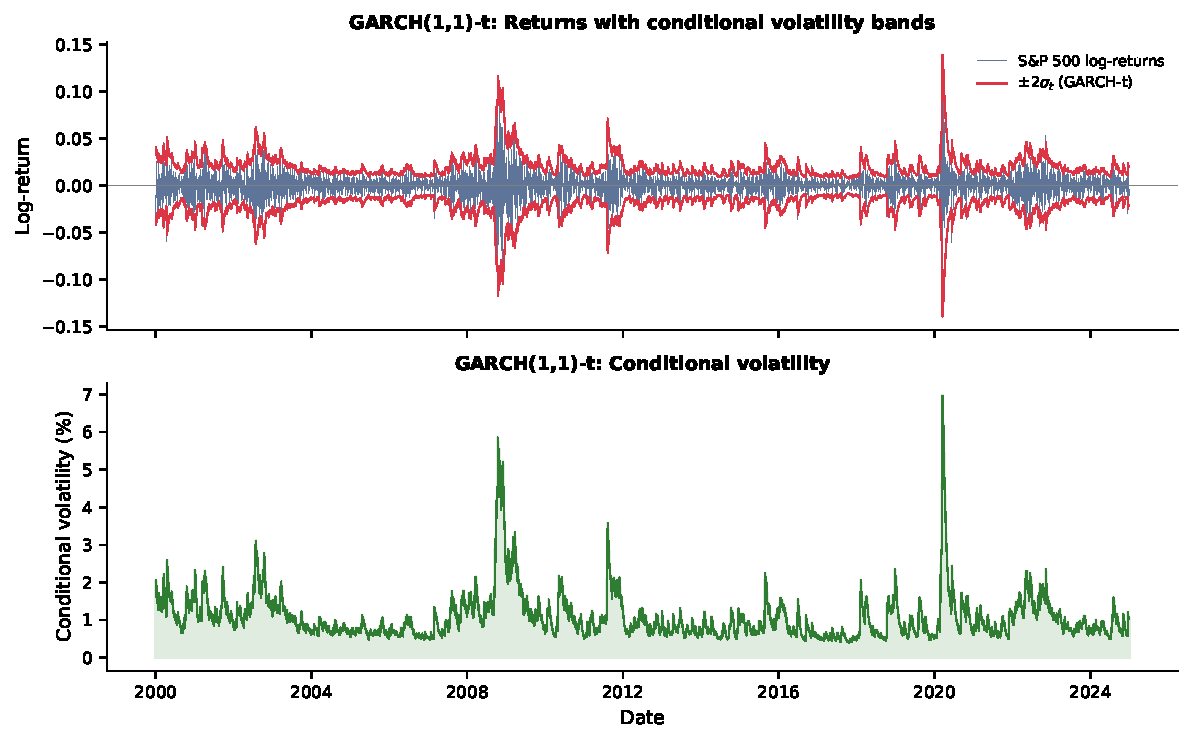
\includegraphics[width=\textwidth]{ch2_garch_t_fit.pdf}
            {\tiny GARCH-$t$: $\sigma_t$ crește în perioade turbulente}
        \end{column}
    \end{columns}
    \quantlet{SFM\_ch2\_modern\_extensions}{https://github.com/QuantLet/Stat_fin_markets/tree/master/Ch_02/SFM_ch2_modern_extensions}
    \end{cminipage}
\end{frame}

\begin{frame}{Exercițiul 4: Rolling VaR --- 3 modele}
    \begin{cminipage}{0.95\textwidth}
    \begin{itemize}\setlength{\itemsep}{0pt}
        \item \textbf{Problemă:} VaR rolling (250 zile) pe $T = 500$ zile out-of-sample, VaR la 1\%:
    \end{itemize}

    \renewcommand{\arraystretch}{1.2}
    \begin{center}
    \begin{tabular}{lccc}
    \toprule
    \textbf{Model} & \textbf{Excepții} & $\hat{p}$ & \textbf{Basel} \\
    \midrule
    Normal & 14 & 2.80\% & ? \\
    Student-$t$ & 6 & 1.20\% & ? \\
    GARCH-$t$ & 4 & 0.80\% & ? \\
    \bottomrule
    \end{tabular}
    \end{center}

    \begin{itemize}\setlength{\itemsep}{0pt}
        \item Calculați LR Kupiec pentru fiecare și clasificați Basel (normalizat la 250 zile).
    \end{itemize}
    \end{cminipage}
\end{frame}

\begin{frame}{Exercițiul 4: Soluție}
    \begin{cminipage}{0.95\textwidth}
    \begin{columns}[T]
        \begin{column}{0.52\textwidth}
            \begin{itemize}\setlength{\itemsep}{0pt}
                \item Așteptat: $T\alpha = 500 \times 0.01 = 5$
            \end{itemize}

            \vspace{0.2cm}
            \renewcommand{\arraystretch}{1.2}
            \begin{tabular}{lccc}
            \toprule
            \textbf{Model} & LR & p-val & \textbf{Decizie} \\
            \midrule
            Normal & 12.5 & 0.0004 & \textcolor{Crimson}{Respins} \\
            Student-$t$ & 0.18 & 0.67 & \textcolor{Forest}{Acceptat} \\
            GARCH-$t$ & 0.43 & 0.51 & \textcolor{Forest}{Acceptat} \\
            \bottomrule
            \end{tabular}

            \vspace{0.2cm}
            \begin{itemize}\setlength{\itemsep}{0pt}
                \item \textbf{Basel (250 zile):}
                \begin{itemize}\setlength{\itemsep}{0pt}
                    \item Normal: $14/2 = 7$ $\Rightarrow$ \textcolor{Amber}{Galben}
                    \item Student-$t$: $6/2 = 3$ $\Rightarrow$ \textcolor{Forest}{Verde}
                    \item GARCH-$t$: $4/2 = 2$ $\Rightarrow$ \textcolor{Forest}{Verde}
                \end{itemize}
            \end{itemize}
        \end{column}
        \begin{column}{0.45\textwidth}
            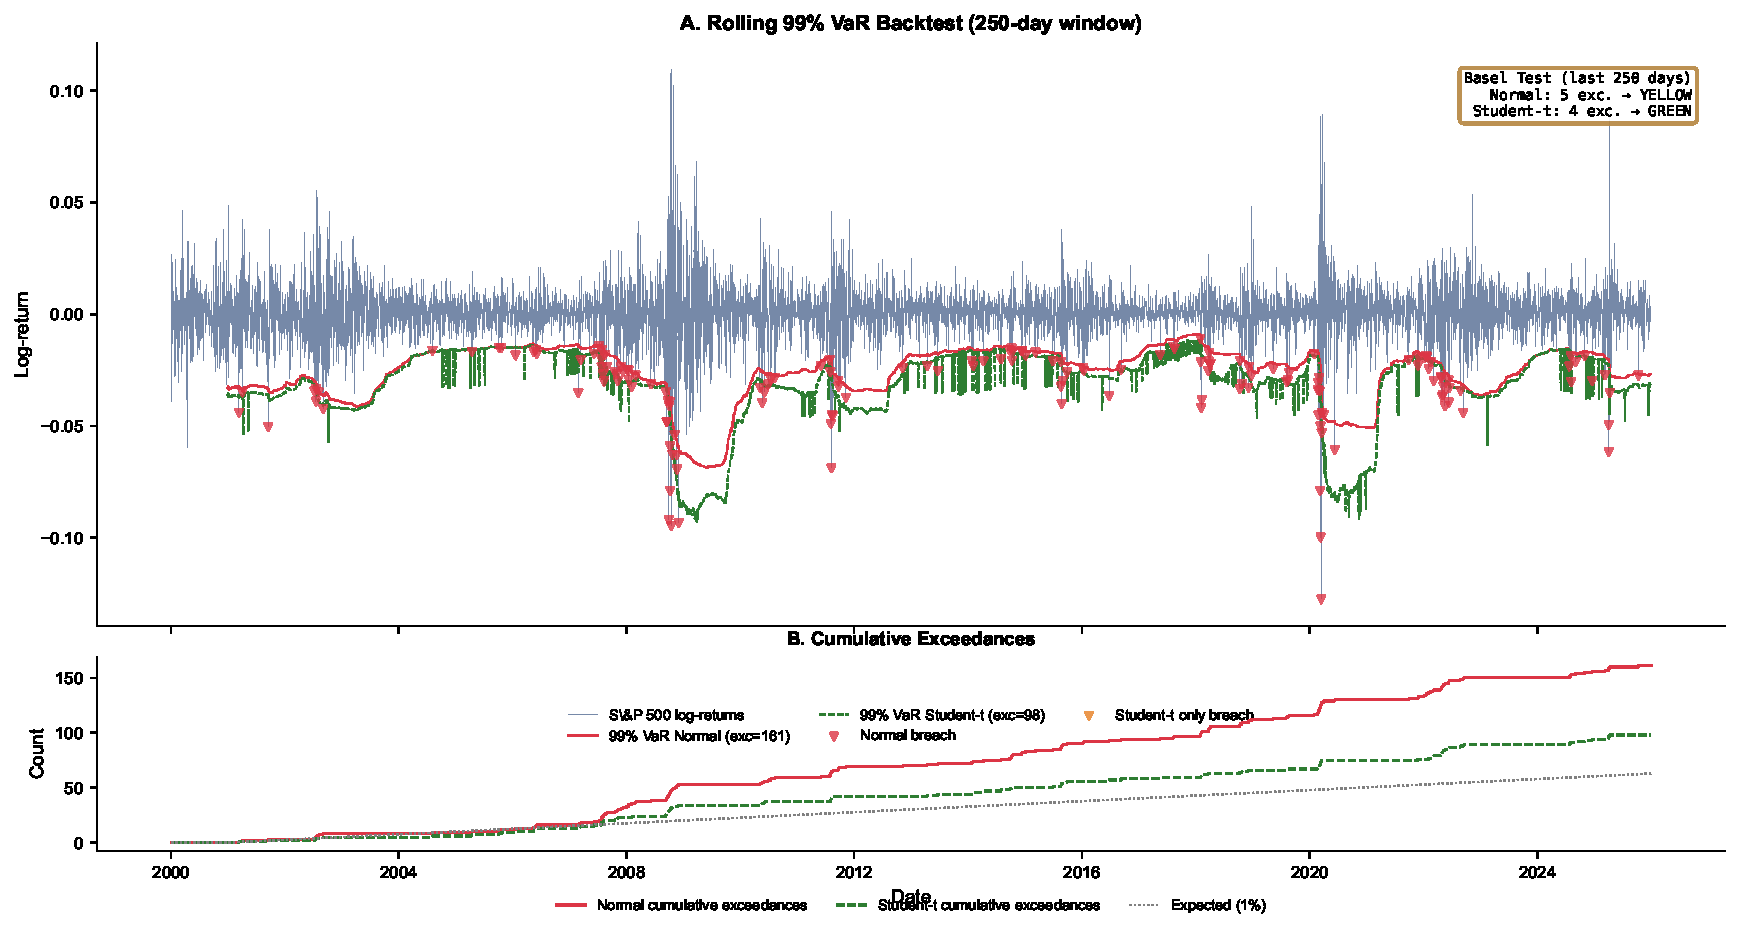
\includegraphics[width=\textwidth]{ch2_var_backtest.pdf}
            {\tiny Backtesting: Normal vs Student-$t$ vs GARCH-$t$}
        \end{column}
    \end{columns}
    \quantlet{SFM\_ch2\_risk\_management}{https://github.com/QuantLet/Stat_fin_markets/tree/master/Ch_02/SFM_ch2_risk_management}
    \end{cminipage}
\end{frame}

%=============================================================================
% PART 4: PYTHON EXERCISES
%=============================================================================
\section{Exerciții Python}

\begin{frame}[fragile]{Exercițiu Python 1: Fit 6 distribuții și clasament AIC}
    \textbf{Sarcină:}
    \begin{enumerate}\setlength{\itemsep}{0pt}
        \item Ajustați Normal, Student-$t$, GED, Laplace, Cauchy, Logistic
        \item Calculați AIC/BIC pentru fiecare
        \item Afișați clasamentul și selectați cel mai bun model
    \end{enumerate}

    \vspace{0.3cm}
    \textbf{Cod cheie:}
    \begin{verbatim}
from scipy import stats
from scipy.stats import gennorm
models = {}
models['Normal'] = {'k':2, 'll': np.sum(stats.norm.logpdf(r, *stats.norm.fit(r)))}
models['Student-t'] = {'k':3, 'll': np.sum(stats.t.logpdf(r, *stats.t.fit(r)))}
models['GED'] = {'k':3, 'll': np.sum(gennorm.logpdf(r, *gennorm.fit(r)))}
    \end{verbatim}

    \quantlet{SFM\_ch2\_distribution\_comparison}{https://github.com/QuantLet/Stat_fin_markets/tree/master/Ch_02/SFM_ch2_distribution_comparison}
\end{frame}

\begin{frame}[fragile]{Exercițiu Python 2: Rolling VaR și testul Kupiec}
    \textbf{Sarcină:}
    \begin{enumerate}\setlength{\itemsep}{0pt}
        \item Implementați VaR rolling (fereastră 250 zile) sub Normal și Student-$t$
        \item Numărați excepțiile și aplicați testul Kupiec
        \item Clasificați conform Basel Traffic Light
    \end{enumerate}

    \vspace{0.3cm}
    \textbf{Cod cheie:}
    \begin{verbatim}
def kupiec_test(x, T, alpha):
    p_hat = x / T
    lr = -2*(x*np.log(alpha/p_hat) + (T-x)*np.log((1-alpha)/(1-p_hat)))
    return lr, 1 - stats.chi2.cdf(lr, df=1)
    \end{verbatim}

    \quantlet{SFM\_ch2\_risk\_management}{https://github.com/QuantLet/Stat_fin_markets/tree/master/Ch_02/SFM_ch2_risk_management}
\end{frame}

\begin{frame}[fragile]{Exercițiu Python 3: GARCH(1,1)-$t$ cu \texttt{arch}}
    \textbf{Sarcină:}
    \begin{enumerate}\setlength{\itemsep}{0pt}
        \item Estimați GARCH(1,1)-$t$ cu pachetul \texttt{arch}
        \item Extrageți volatilitatea condiționată
        \item Calculați VaR condiționat și vizualizați backtesting
    \end{enumerate}

    \vspace{0.3cm}
    \textbf{Funcții cheie:}
    \begin{itemize}\setlength{\itemsep}{0pt}
        \item \texttt{arch\_model(r\_pct, vol='Garch', p=1, q=1, dist='t')}
        \item \texttt{result.params} pentru $\omega, \alpha, \beta, \nu$
        \item \texttt{result.conditional\_volatility} pentru $\sigma_t$
        \item VaR: $\hat{\mu} + \hat{\sigma}_t \cdot t_\nu^{-1}(\alpha)$
    \end{itemize}

    \quantlet{SFM\_ch2\_modern\_extensions}{https://github.com/QuantLet/Stat_fin_markets/tree/master/Ch_02/SFM_ch2_modern_extensions}
\end{frame}

%=============================================================================
% PART 5: DISCUSSION QUESTIONS
%=============================================================================
\section{Întrebări de Discuție}

\begin{frame}{Discuție 1: Alegerea modelului pentru reglementare}
    \begin{cminipage}{0.95\textwidth}
    \begin{itemize}\setlength{\itemsep}{0pt}
        \item \textbf{Scenariu:} O bancă poate folosi VaR Normal static (simplu, zona galben Basel) sau GARCH-$t$ (complex, zona verde Basel). Departamentul IT preferă normalul, departamentul de risc preferă GARCH-$t$.
    \end{itemize}

    \vspace{0.3cm}
    \begin{itemize}\setlength{\itemsep}{0pt}
        \item \textbf{Întrebări:}
    \end{itemize}
    \begin{enumerate}\setlength{\itemsep}{0pt}
        \item Ce argumente are fiecare departament?
        \item Care sunt costurile zonei galben vs verde (multiplicator $k$)?
        \item Este GARCH-$t$ întotdeauna superior?
        \item Ce alte considerații practice sunt relevante?
    \end{enumerate}
    \end{cminipage}
\end{frame}

\begin{frame}{Discuție 2: Diversificarea în criză}
    \begin{cminipage}{0.95\textwidth}
    \begin{itemize}\setlength{\itemsep}{0pt}
        \item \textbf{Scenariu:} Portofoliu diversificat: S\&P 500 + EURUSD + Aur. Corelația Pearson: 0.3. Copula Gaussiană: $\lambda_L = 0$. Copula Student-$t$($\nu = 4$): $\lambda_L = 0.15$.
    \end{itemize}

    \vspace{0.3cm}
    \begin{itemize}\setlength{\itemsep}{0pt}
        \item \textbf{Întrebări:}
    \end{itemize}
    \begin{enumerate}\setlength{\itemsep}{0pt}
        \item Ce semnifică $\lambda_L = 0.15$ pentru portofoliu?
        \item Diversificarea funcționează în criză? De ce?
        \item Cum ați modifica alocarea ținând cont de dependența de coadă?
        \item Ce instrumente de hedging sunt eficiente?
    \end{enumerate}

    \vspace{0.3cm}
    \begin{itemize}\setlength{\itemsep}{0pt}
        \item \textbf{Indiciu:} Gândiți-vă la criza din 2008 și la co-crashul activelor ``necorelate''.
    \end{itemize}
    \end{cminipage}
\end{frame}

%=============================================================================
% EXERCIȚIU CU ASISTENȚĂ AI
%=============================================================================
\section{Exercițiu cu asistență AI}

\begin{frame}{Exercițiu AI: Gândire critică}
    \begin{cminipage}{0.95\textwidth}
    \vspace{-3mm}
    \begin{block}{\footnotesize Prompt de testat în ChatGPT / Claude / Copilot}
        {\footnotesize
        ``Descarcă de pe Yahoo Finance datele zilnice S\&P 500 din 2015 până în 2025. Calculează log-randamentele. Ajustează 6 distribuții (Normal, Student-t, GED, Laplace, Cauchy, Logistic) prin MLE. Compară AIC/BIC. Implementează VaR rolling pe 250 zile sub Normal și Student-t. Aplică testul Kupiec. Estimează GARCH(1,1)-t cu pachetul arch. Vizualizează backtesting. Vreau cod Python complet.''
        }
    \end{block}
    \vspace{-2mm}
    {\footnotesize
    \begin{itemize}\setlength{\itemsep}{0pt}
        \item \textbf{Exercițiu}:
    \end{itemize}
    \begin{enumerate}\setlength{\itemsep}{0pt}
        \item Rulați prompt-ul într-un LLM la alegere și analizați critic răspunsul.
        \item Testul Kupiec este implementat corect (formula LR, nu doar contorizare)?
        \item GARCH-$t$ folosește \texttt{dist='t'} sau implicit normală?
        \item VaR-ul GARCH folosește cuantila $t_\nu$ sau $\Phi^{-1}$?
        \item Graficul de backtesting marchează excepțiile vizual?
    \end{enumerate}
    }
    \vspace{-2mm}
    \begin{alertblock}{}
        {\footnotesize \textbf{Atenție}: Codul generat de AI poate rula fără erori și arăta profesional. \textit{Asta nu înseamnă că e corect.}}
    \end{alertblock}
    \end{cminipage}
\end{frame}

%=============================================================================
% SUMMARY
%=============================================================================
\section{Rezumat}

\begin{frame}{Concluzii Cheie de Astăzi}
    \begin{cminipage}{0.95\textwidth}
    \begin{enumerate}\setlength{\itemsep}{0pt}
        \item \textbf{AIC/BIC selectează modelul} --- $\Delta > 10$ este ``foarte semnificativ''
        \item \textbf{Testul LR compară} modele nested --- $\text{LR} = -2(\ell_0 - \ell_1) \sim \chi^2(\Delta k)$
        \item \textbf{Backtesting validează} modelul pe date out-of-sample, nu in-sample
        \item \textbf{Kupiec test}: $H_0$: rata excepțiilor $= \alpha$; respingere $\Rightarrow$ model inadecvat
        \item \textbf{GARCH-$t$ captează} volatility clustering + cozi grele simultan
        \item \textbf{Basel Traffic Light}: $\leq 4$ exc./250 zile = verde; 5--9 = galben; $\geq 10$ = roșu
    \end{enumerate}

    \vspace{0.3cm}
    \begin{block}{Următorul Seminar}
        \begin{itemize}\setlength{\itemsep}{0pt}
            \item Ipoteza Piețelor Eficiente
        \end{itemize}
    \end{block}
    \end{cminipage}
\end{frame}

%=============================================================================
% REFERINȚE
%=============================================================================
\begin{frame}{Bibliografie I}
    \begin{cminipage}{0.95\textwidth}
    \begin{block}{Selecția Modelului și Backtesting}
        {\small
        \begin{itemize}\setlength{\itemsep}{0pt}
            \item Kupiec, P. (1995). ``Techniques for verifying the accuracy of risk measurement models,'' \textit{Journal of Derivatives}, 3(2).
            \item Christoffersen, P. (1998). ``Evaluating interval forecasts,'' \textit{International Economic Review}, 39(4), 841--862.
            \item Bollerslev, T. (1986). ``Generalized autoregressive conditional heteroskedasticity,'' \textit{Journal of Econometrics}, 31, 307--327.
            \item Basel Committee on Banking Supervision (1996). ``Supervisory framework for the use of `backtesting','' BIS.
        \end{itemize}
        }
    \end{block}
    \end{cminipage}
\end{frame}

\begin{frame}{Surse de Date și Software}
    \begin{cminipage}{0.95\textwidth}
    \begin{block}{Instrumente Software}
        {\small
        \begin{itemize}\setlength{\itemsep}{0pt}
            \item \texttt{scipy.stats} --- Distribuții parametrice, teste statistice
            \item \texttt{arch} --- Modele GARCH, distribuții condiționale
            \item \texttt{yfinance} --- Descărcare date financiare
            \item \texttt{matplotlib}, \texttt{seaborn} --- Vizualizare
        \end{itemize}
        }
    \end{block}

    \vspace{0.3cm}
    \begin{block}{Date și Exemple}
        {\small
        \begin{itemize}\setlength{\itemsep}{0pt}
            \item S\&P 500, BET, Bitcoin --- descărcate via \texttt{yfinance}
            \item Notebook-uri Jupyter disponibile pe GitHub (QuantLet)
        \end{itemize}
        }
    \end{block}
    \end{cminipage}
\end{frame}

\begin{frame}{Exercițiu de Replicare: Kupiec (1995)}
    \begin{cminipage}{0.95\textwidth}
        \begin{block}{Obiectiv}
            \begin{itemize}\setlength{\itemsep}{0pt}
                \item Replicați tabelul principal din Kupiec (1995): frecvența excepțiilor VaR pe date simulate și reale.
            \end{itemize}
        \end{block}
        \begin{enumerate}\setlength{\itemsep}{2pt}
            {\small
            \item Descărcați randamentele zilnice S\&P 500 (ultimii 10 ani)
            \item Implementați VaR rolling (250 zile) sub Normal, Student-$t$ și GARCH-$t$
            \item Numărați excepțiile la 1\% și 5\% pentru fiecare model
            \item Aplicați testul Kupiec pe fiecare combinație model/nivel
            \item Clasificați fiecare model conform Basel Traffic Light
            \item \textbf{Întrebare}: Ce model obține zona \textcolor{Forest}{verde} pe cele mai multe sub-perioade?
            }
        \end{enumerate}
        {\tiny Ref: Kupiec, P. (1995). ``Techniques for verifying the accuracy of risk measurement models,'' \textit{Journal of Derivatives}, 3(2).}
    \end{cminipage}
\end{frame}

\begin{frame}{Temă pentru acasă: Seminar 4}
    \begin{cminipage}{0.95\textwidth}
    \begin{block}{Obiectiv}
        \begin{itemize}\setlength{\itemsep}{0pt}
            \item Implementați un sistem complet de backtesting VaR.
        \end{itemize}
    \end{block}
    \begin{enumerate}\setlength{\itemsep}{2pt}
        {\small
        \item Descărcați randamentele zilnice S\&P 500 (ultimii 10 ani)
        \item Implementați VaR rolling (fereastra 250 zile) sub 4 distribuții: Normal, Student-$t$, Skew-$t$, GARCH(1,1)-$t$
        \item Numărați excepțiile la nivelurile 1\% și 5\%
        \item Aplicați testul Kupiec (LR) pe fiecare combinație
        \item Clasificați conform Basel Traffic Light (verde/galben/roșu)
        \item Vizualizați: randamente + VaR rolling + excepții marcate
        \item \textbf{Întrebare}: Ce model obține zona \textcolor{Forest}{verde} pe cele mai multe sub-perioade?
        }
    \end{enumerate}
    \quantlet{SFM\_ch2\_case\_study\_2c}{https://github.com/QuantLet/Stat_fin_markets/tree/master/Ch_02/SFM_ch2_case_study_2c}
    \end{cminipage}
\end{frame}

\begin{frame}{}
    \begin{cminipage}{0.95\textwidth}
    \centering
    \Huge\textcolor{IDAred}{Vă mulțumesc!}
    \vspace{1cm}
    \Large\textcolor{MainBlue}{Întrebări?}
    \vspace{0.8cm}
    \normalsize
    Materialele seminarului sunt disponibile la: \url{https://danpele.github.io/SFM/}
    \vspace{0.2cm}
    \href{https://quantlet.com}{\raisebox{-0.15em}{
\includegraphics[height=0.8em]{ql_logo.png}} Quantlet} \hspace{0.5cm}
    \href{https://quantinar.com}{\raisebox{-0.15em}{
\includegraphics[height=0.8em]{qr_logo.png}} Quantinar}
    \end{cminipage}
\end{frame}

\end{document}
